% Options for packages loaded elsewhere
\PassOptionsToPackage{unicode}{hyperref}
\PassOptionsToPackage{hyphens}{url}
\PassOptionsToPackage{dvipsnames,svgnames,x11names}{xcolor}
%
\documentclass[
  authoryear,
  preprint,
  3p,
  onecolumn]{elsarticle}

\usepackage{amsmath,amssymb}
\usepackage{iftex}
\ifPDFTeX
  \usepackage[T1]{fontenc}
  \usepackage[utf8]{inputenc}
  \usepackage{textcomp} % provide euro and other symbols
\else % if luatex or xetex
  \usepackage{unicode-math}
  \defaultfontfeatures{Scale=MatchLowercase}
  \defaultfontfeatures[\rmfamily]{Ligatures=TeX,Scale=1}
\fi
\usepackage{lmodern}
\ifPDFTeX\else  
    % xetex/luatex font selection
\fi
% Use upquote if available, for straight quotes in verbatim environments
\IfFileExists{upquote.sty}{\usepackage{upquote}}{}
\IfFileExists{microtype.sty}{% use microtype if available
  \usepackage[]{microtype}
  \UseMicrotypeSet[protrusion]{basicmath} % disable protrusion for tt fonts
}{}
\makeatletter
\@ifundefined{KOMAClassName}{% if non-KOMA class
  \IfFileExists{parskip.sty}{%
    \usepackage{parskip}
  }{% else
    \setlength{\parindent}{0pt}
    \setlength{\parskip}{6pt plus 2pt minus 1pt}}
}{% if KOMA class
  \KOMAoptions{parskip=half}}
\makeatother
\usepackage{xcolor}
\setlength{\emergencystretch}{3em} % prevent overfull lines
\setcounter{secnumdepth}{5}
% Make \paragraph and \subparagraph free-standing
\ifx\paragraph\undefined\else
  \let\oldparagraph\paragraph
  \renewcommand{\paragraph}[1]{\oldparagraph{#1}\mbox{}}
\fi
\ifx\subparagraph\undefined\else
  \let\oldsubparagraph\subparagraph
  \renewcommand{\subparagraph}[1]{\oldsubparagraph{#1}\mbox{}}
\fi


\providecommand{\tightlist}{%
  \setlength{\itemsep}{0pt}\setlength{\parskip}{0pt}}\usepackage{longtable,booktabs,array}
\usepackage{calc} % for calculating minipage widths
% Correct order of tables after \paragraph or \subparagraph
\usepackage{etoolbox}
\makeatletter
\patchcmd\longtable{\par}{\if@noskipsec\mbox{}\fi\par}{}{}
\makeatother
% Allow footnotes in longtable head/foot
\IfFileExists{footnotehyper.sty}{\usepackage{footnotehyper}}{\usepackage{footnote}}
\makesavenoteenv{longtable}
\usepackage{graphicx}
\makeatletter
\def\maxwidth{\ifdim\Gin@nat@width>\linewidth\linewidth\else\Gin@nat@width\fi}
\def\maxheight{\ifdim\Gin@nat@height>\textheight\textheight\else\Gin@nat@height\fi}
\makeatother
% Scale images if necessary, so that they will not overflow the page
% margins by default, and it is still possible to overwrite the defaults
% using explicit options in \includegraphics[width, height, ...]{}
\setkeys{Gin}{width=\maxwidth,height=\maxheight,keepaspectratio}
% Set default figure placement to htbp
\makeatletter
\def\fps@figure{htbp}
\makeatother

\usepackage{lineno}\linenumbers \usepackage{multirow} \usepackage{lscape} \newcommand{\blandscape}{\begin{landscape}} \newcommand{\elandscape}{\end{landscape}}
\makeatletter
\makeatother
\makeatletter
\makeatother
\makeatletter
\@ifpackageloaded{caption}{}{\usepackage{caption}}
\AtBeginDocument{%
\ifdefined\contentsname
  \renewcommand*\contentsname{Table of contents}
\else
  \newcommand\contentsname{Table of contents}
\fi
\ifdefined\listfigurename
  \renewcommand*\listfigurename{List of Figures}
\else
  \newcommand\listfigurename{List of Figures}
\fi
\ifdefined\listtablename
  \renewcommand*\listtablename{List of Tables}
\else
  \newcommand\listtablename{List of Tables}
\fi
\ifdefined\figurename
  \renewcommand*\figurename{Figure}
\else
  \newcommand\figurename{Figure}
\fi
\ifdefined\tablename
  \renewcommand*\tablename{Table}
\else
  \newcommand\tablename{Table}
\fi
}
\@ifpackageloaded{float}{}{\usepackage{float}}
\floatstyle{ruled}
\@ifundefined{c@chapter}{\newfloat{codelisting}{h}{lop}}{\newfloat{codelisting}{h}{lop}[chapter]}
\floatname{codelisting}{Listing}
\newcommand*\listoflistings{\listof{codelisting}{List of Listings}}
\makeatother
\makeatletter
\@ifpackageloaded{caption}{}{\usepackage{caption}}
\@ifpackageloaded{subcaption}{}{\usepackage{subcaption}}
\makeatother
\makeatletter
\@ifpackageloaded{tcolorbox}{}{\usepackage[skins,breakable]{tcolorbox}}
\makeatother
\makeatletter
\@ifundefined{shadecolor}{\definecolor{shadecolor}{rgb}{.97, .97, .97}}
\makeatother
\makeatletter
\makeatother
\makeatletter
\makeatother
\journal{Journal Name}
\ifLuaTeX
  \usepackage{selnolig}  % disable illegal ligatures
\fi
\usepackage[]{natbib}
\bibliographystyle{elsarticle-harv}
\IfFileExists{bookmark.sty}{\usepackage{bookmark}}{\usepackage{hyperref}}
\IfFileExists{xurl.sty}{\usepackage{xurl}}{} % add URL line breaks if available
\urlstyle{same} % disable monospaced font for URLs
\hypersetup{
  pdftitle={Drought indices of water demand and supply, soil moisture, vegetation, and their impact on LULCC in continental Chile},
  pdfauthor={Francisco Zambrano},
  pdfkeywords={drought, land cover change, satellite},
  colorlinks=true,
  linkcolor={blue},
  filecolor={Maroon},
  citecolor={Blue},
  urlcolor={Blue},
  pdfcreator={LaTeX via pandoc}}

\setlength{\parindent}{6pt}
\begin{document}

\begin{frontmatter}
\title{Drought indices of water demand and supply, soil moisture,
vegetation, and their impact on LULCC in continental Chile}
\author[1]{Francisco Zambrano%
\corref{cor1}%
\fnref{fn1}}
 \ead{francisco.zambrano@umayor.cl} 

\affiliation[1]{organization={Universidad Mayor, Hémera Centro de
Observación de la Tierra, Facultad de Ciencias, Escuela de Ingeniería en
Medio Ambiente y Sustentabilidad},city={Santiago,
Chile},postcode={7500994},postcodesep={}}

\cortext[cor1]{Corresponding author}
\fntext[fn1]{This is the first author footnote.}
        
\begin{abstract}
Central Chile has been the focus of research studies due to the
persistent decrease in water supply, which is impacting the hydrological
system and vegetation development. This persistent period of water
scarcity has been defined as a ``Mega Drought''. Our objective is to
examine the effects of drought on LULCC (land use land cover change)
over continental Chile using drought indices of water supply and demand,
soil moisture, and vegetation productivity. For the analysis,
continental Chile was divided into five zones according to a latitudinal
gradient: ``Norte Grande,'' ``Norte Chico,'' ``Centro,'' ``Sur,'' and
``Austral.'' The monthly ERA5-Land (ERA5L) variables for precipitation,
temperature, and soil moisture were used. From 2001 to 2022, we used the
land cover MODIS product MCD12Q1, and from 2000 to 2023, we used the
NDVI (Normalized Difference Vegetation Index) product MOD13A3 collection
6.1. We estimated atmospheric evaporative demand (AED) using the
Hargreaves-Samani equation with the ERA5L temperature. We used the
Standardized Precipitation Index (SPI), the Standardized Precipitation
Evapotranspiration Index (SPEI), the Evaporative Demand Drought Index
(EDDI), the Standardized Soil Moisture Index (SSI), and the Standardized
anomaly of cumulative NDVI (zcNDVI) as drought indicators. These indices
were calculated for time scales of 1, 3, 6, 12, 24, and 36 months,
except for zcNDVI, which was for 6 months. We analyze the trend for
LULCC, vegetation productivity, and drought indices. Also, we analyzed
the temporal correlation of SPI, SPEI, EDDI, and SSI with zcNDVI to gain
insights into the impact of water supply and demand on vegetation
productivity. Our results showed that LULCC were highest in ``Centro,''
``Sur,'' and ``Austral,'' with 36\%, 31\%, and 34\%, respectively. The
EDDI shows that water demand has increased for all zones, with a major
increase in ``Norte Grande.'' The drought indices of water supply and
soil moisture evidence a decreasing trend, which decreases at longer
time scales, from ``Norte Grande'' to ``Sur.'' ``Austral'' is the only
zone that shows an increase in supply. Vegetation productivity measures
by zcNDVI present a negative trend in ``Norte Chico'' and ``Centro.''
Showing to be the zones most impacted by climatic conditions, the years
2020 and 2022 suffered the most extreme drought. On the other hand,
forests seem to be the most resistant to drought. The types that show to
be most affected by variation in climate conditions are shrublands,
savannas, and croplands. The drought indices that have the capability of
explaining to a major degree the variance in vegetation productivity are
SSI-12, followed by SPEI-24 and SPEI-12 in ``Norte Chico'' and
``Centro.'' The results indicate that ``Norte Chico'' and ``Zona
Central'' are the most sensitive regions to water supply deficits longer
than a year, potentially explained by a low capacity of water storage in
those zones that should be further investigated.
\end{abstract}





\begin{keyword}
    drought \sep land cover change \sep 
    satellite
\end{keyword}
\end{frontmatter}
    \captionsetup{justification=raggedright,singlelinecheck=false}

\ifdefined\Shaded\renewenvironment{Shaded}{\begin{tcolorbox}[borderline west={3pt}{0pt}{shadecolor}, breakable, boxrule=0pt, sharp corners, frame hidden, interior hidden, enhanced]}{\end{tcolorbox}}\fi

\hypertarget{introduction}{%
\section{Introduction}\label{introduction}}

The sixth assessment report (AR6) of the IPCC \citep{IPCC2023} indicates
that human-induced greenhouse gas emissions have increased the frequency
and/or intensity of some weather and climate extremes, and the evidence
has been strengthened since AR5 \citep{IPCC2013}. There is a high degree
of confidence that rising temperatures will increase the land area where
droughts will occur more frequently and with greater severity
\citep{IPCCCH112021}. Furthermore, drought increases tree mortality and
triggers changes in land cover and, consequently, land use, thus
impacting ecosystems \citep{Crausbay2017}. Nevertheless, there is a lack
of understanding of how the alteration in water supply and demand is
affecting land cover transformations.

The primary cause of drought is precipitation, and temperature makes it
worse \citep{Luo2017}. Drought impacts soil moisture, hydrological
regimes, and vegetation productivity. Initially, drought was commonly
classified as meteorological, hydrological, and agricultural
\citep{Wilhite1985}. Lately, \citet{Loon2016} and
\citet{AghaKouchak2021} have given an updated definition of drought for
the Anthropocene, suggesting that it should be considered the feedback
of humans' decisions and activities that drives the anthropogenic
drought. Even though it has been argued that those definitions do not
fully address the ecological dimensions of drought, \citet{Crausbay2017}
proposed the ecological drought definition as ``an episodic deficit in
water availability that drives ecosystems beyond thresholds of
vulnerability, impacts ecosystem services, and triggers feedback in
natural and/or human systems.''. Moreover, many ecological studies have
misinterpreted how to characterize drought, for example, sometimes
considering ``dry'' conditions as ``drought'' \citep{Slette2019}. On the
other hand, the AR6 \citep{IPCC2023} predicts that many regions of the
world will experience more severe agricultural and ecological droughts
even if global warming stabilizes at 1.5°--2°C. Then, there is a
challenge in conducting drought research, especially to evaluate its
impact on ecosystems.

Chile has been facing a persistent rainfall deficit for more than a
decade \citep{Garreaud2017}, which has impacted vegetation development
\citep{Zambrano2023} and the hydrological system \citep{Boisier2018}.
Current drought conditions have affected crop productivity
\citep{Zambrano2016, Zambrano2018}, forest development
\citep{Miranda2020, Venegas2018}, forest fire occurrence
\citep{UrrutiaJalabert2018}, land cover change \citep{Fuentes2021},
water supply in watersheds \citep{AlvarezGarreton2021}, and have had
economic impacts \citep{Fernandez2023}. In 2019--2020, the drought
severity reached an extreme condition in Central Chile (30--34°S) not
seen for at least 40 years, and the evidence indicates that the impact
is transversal to the land cover classes of forest, grassland, and
cropland \citep{Zambrano2023}. The prolonged lack of precipitation in
Central Chile is producing changes in ecosystem dynamics that must be
studied.

For the spatiotemporal assessment of drought impact (i.e., by water
supply and demand) on land cover changes, we need climatic realiable
variables such as precipitation, temperature, soil moisture, land cover,
and vegetation status. For developing countries like Chile, the weather
networks present several disadvantages, such as gaps, a short history,
and low-quality data. Reanalysis data, as the ERA5-Land (ERA5L)
\citep{MunozSabater2021} provides hourly climatic information
(precipitation, temperature, and soil moisture) without gaps since 1950
with global extension. ERA5L has already been used for drought
assessment using the Standardized Precipitation-Evapotranspiration Index
(SPEI) \citep{Nouri2023} and for flash drought \citep{Wang2023} by
analyzing soil moisture and evapotranspiration. On the other hand,
satellite remote sensing \citep{West2019, AghaKouchak2015} is the
primary method to evaluate how drought impacts vegetation dynamics. The
Moderate-Resolution Imaging Spectroradiometer (MODIS) can be used to get
vegetation drought indices (VDI), which are often used as proxies for
productivity \citep{Paruelo2016, Schucknecht2017}. Besides, land use and
land cover (LULC) change can be driven by drought
\citep{Tran2019, Akinyemi2021}. To analyze these changes, multiple LULC
products exist \citep{Grekousis2015}. One of those that provides time
series since 2001 is the MCD12Q1 \citep{Friedl2019} from MODIS. The
variation in water supply and demand is finally reflected in the total
water storage (TWS). The Gravity Recovery and Climate Experiment
(GRACE), which allows analyzing changes in water availability at coarse
resolution, can retrieve the TWS \citep{Ahmed2014, Ma2017}. We can find
drought indices of supply (i.e., precipitation) and demand (i.e.,
temperature) using climatic reanalysis (ERA5L) and vegetation data
(MODIS). This lets us figure out how drought changes LULC. Further, the
TWS can be assessed with regard to the changes in water supply and
demand to gain insight into the impact on water storage.

To evaluate meteorological drought (i.e., water supply), the World
Meteorological Organization (WMO; \citet{WMO2012}) recommends the
Standardized Precipitation Index (SPI; \citet{Mckee1993}), a multiscalar
drought index that allows to monitor precipitation deficits from short-
to long-term. Following the same approach, \citet{Vicente-Serrano2010}
incorporates into the SPI the effect of temperature through the use of
potential evapotranspiration, thus proposing the SPEI (Standardized
Precipitation Evapotranspiration Index). Similarly, to evaluate solely
the evaporative demand driven by temperature, \citet{Hobbins2016} and
\citet{McEvoy2016} came up with the Evaporative Demand Drought Index
(EDDI). For vegetation, in a similar manner as the SPI, SPEI and EDDI;
\citet{Zambrano2018} proposed the zcNDVI, a standardized anomaly of the
cumulative Normalized Difference Vegetation Index (NDVI), which could be
acumulated over the growing season or any period (e.g., months),
resulting in a multiscalar drought index. For soil moisture, several
drought indices exist, such as the Soil Moisture Deficit Index (SDMI) a
normalized index \citep{Narasimhan2005} and the Soil Moisture
Agricultural Drought Index (SMADI) \citep{Souza2021} which is a
normalized index using vegetation, land surface temperature, and a
vegetation condition index (VCI, \citep{Kogan1995}). From TWS, we can
estimate the standardized terrestrial water storage index (STI)
\citep{Cui2021}, a standardized anomaly that follows the methodology of
the SPI, SPEI, EDDI, and zcNDVI. Thereby, we have drought indices for
water supply, demand, and storage, which can help to make a
comprehensive assessment of drought.

In this research, we aim to analyze the impact of drought on different
types of ecosystems (land cover classes) in continental Chile. Our
specific goals are: i) to analyze the trend on multi-scalar drought
indices for water demand and supply, soil moisture, and vegetation
productivity for 1981--2023/2001--2023; ii) to assess the LULC change
for 2001--2021 and how it relates to drought indices; iii) to evaluate
the relationship between zcNDVI, a measure of vegetation productivity,
and drought indices for water demand and supply and soil moisture; and
iv) to assess if the observed changes in the drought indices are linked
to TWS.

\hypertarget{study-area}{%
\section{Study area}\label{study-area}}

Continetal Chile has a diverse climate condition from north to south and
east to west \citep{Aceituno2021} (Figure~\ref{fig-studyArea}), which
determines its great ecosystem diversity (Figure~\ref{fig-LCprop}). The
Andes Mountains are a main factor in latitudinal variation
\citep{Garreaud2009}. To describe the climate and ecosystem of Chile, we
use the Koppen-Geiger release by \citet{Beck2023} and the land cover
type persistance of 80\% of times for 2001--2022, from the IGBP
classification scheme \citep{Friedl2019} (see
Section~\ref{sec-methods_lulc}). ``Norte Grande'' and ``Norte Chico''
predominate in an arid desert climate with hot (Bwh) and cold (Bwk)
temperatures. At the south of ``Norte Chico,'' the climate changes to an
arid steppe with cold temperatures (Bsk). Mainly, the land is barren,
with a minor surface of vegetation types such as shrubland and
grassland. In the zones ``Centro'' and the north half of ``Sur,'' the
main climate is Mediterranean, with warmer to hot summers (Csa and Csb).
There is a significant amount (50\%) of Chilean matorral (shrubland and
savanna, \citep{Fuentes2021}), then grassland (16\%), forest (8\%), and
croplands (5\%), in ``Centro.'' The south part of ``Sur'' and the north
part of ``Austral'' are dominated by an oceanic climate (Cfb). Those
zones are high in forest and grassland. The southern part of the country
has a tundra climate, and in Patagonia, it is a cold semi-arid area with
an extended surface of grassland, forest, and, to a lesser extent,
savanna.

\begin{figure*}[!ht]

{\centering 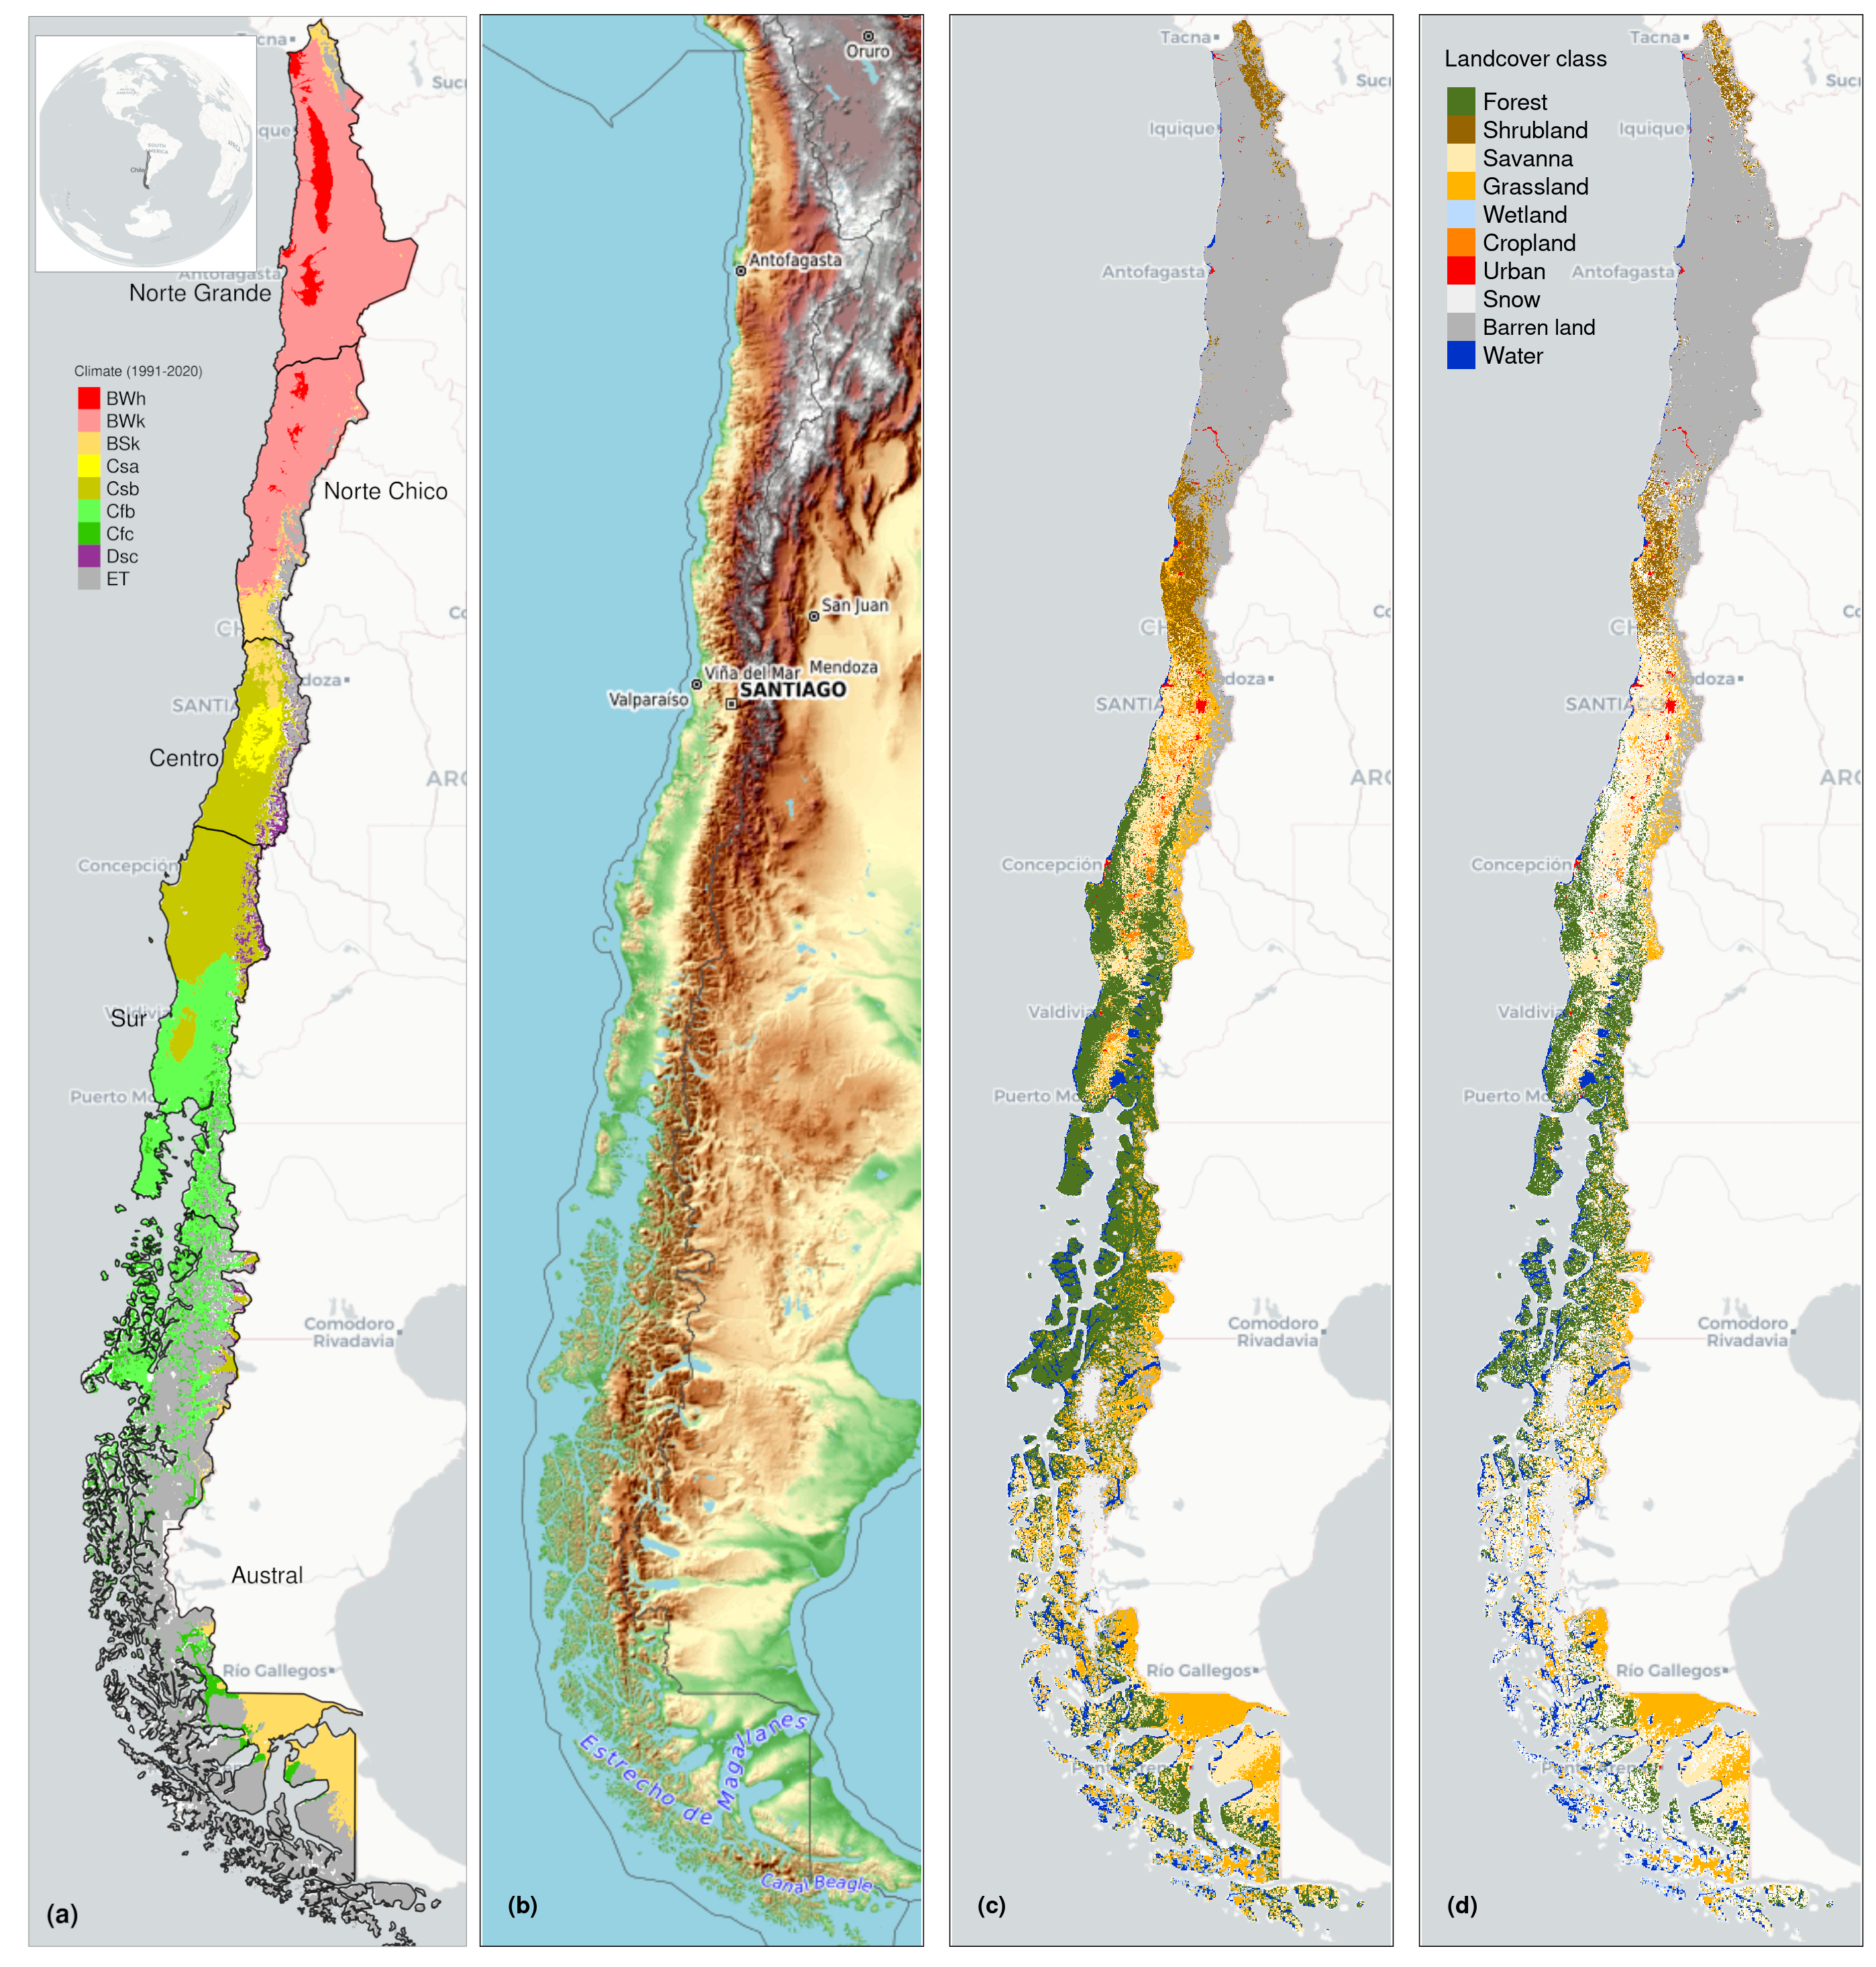
\includegraphics{../output/figs/map_study_con_landcover.png}

}

\caption{\label{fig-studyArea}(a) Chile with the Koppen-Geiger climate
classes and the five macrozones ``Norte Grande'', ``Norte Chico'',
``Centro'', ``Sur'', and ``Austral''. (b) Topography reference map. (c)
Land cover classes for 2022. (d) Persistent land cover classes
(\textgreater{} 80\%) for 2001-2022}

\end{figure*}

\hypertarget{materials-and-methods}{%
\section{Materials and Methods}\label{materials-and-methods}}

\hypertarget{software-and-packages-used}{%
\subsection{Software and packages
used}\label{software-and-packages-used}}

For the downloading, processing, and analysis of the spatio-temporal
data, we used the open source software for statistical computing and
graphics, \texttt{R} \citep{R2023}. For downloading ERA5L, we used the
\texttt{\{ecmwfr\}} package \citep{Hufkens2019}. For processing raster
data, we used \texttt{\{terra\}} \citep{Hijmans2023} and
\texttt{\{stars\}} \citep{Pebesma2023}. For managing vectorial data, we
used \texttt{\{sf\}} \citep{Pebesma2018}. For the calculation of AED, we
used \texttt{\{SPEI\}} \citep{Bergueria2023}.

\hypertarget{data}{%
\subsection{Data}\label{data}}

\hypertarget{earth-observation-data}{%
\subsubsection{Earth observation data}\label{earth-observation-data}}

For water supply and demand variables, we used ERA5L
\citep{MunozSabater2021}, a reanalys dataset that provides the evolution
of land variables since 1950. It has a spatial resolution of 0.1°,
hourly frequency, and global coverage. We selected the variables for
total precipitation, 2 meter temperature maximum and minimum, and
volumetric soil water layers between 0 and 100cm of depth (layer 1 to
layer 3). The data was downloaded using the Copernicus Climate Data
Store (CDS) Application Program Interface (API) implemented in
\texttt{\{ecmfwr\}} \citep{Hufkens2019}.

To derive a proxy of vegetation productivity, we used the product
MOD13A3 collection 6.1 from MODIS \citep{Didan2015}. It provides
vegetation indices (NDVI and EVI) at 1km of spatial resolution and
monthly frequency. The MOD13A3.061 and MCD12Q1.061 were retrieved from
the online Data Pool, courtesy of the NASA EOSDIS Land Processes
Distributed Active Archive Center (LP DAAC), USGS Earth Resources
Observation and Science (EROS) Center, Sioux Falls, South Dakota,
https://lpdaa.usgs.gov/tools/data-pool/.

\begin{table}[!ht]
\caption{Description of the earth observation data used }
\label{tab-desEOD}
\small
\centering
\begin{tabular}{p{0.13\textwidth}cp{0.3\textwidth}p{0.095\textwidth}ccc}
\hline
\multirow{1}{*}{\centering Product} & Sub-product & Variable & Spatial Resolution  & Period & Units & Short Name \\ 
\hline
\multirow{4}{*}{ERA5L} & ~ & Precipitation & \multirow{4}{*}{~0.1°} & \multirow{4}{*}{1981-2023} & mm & P \\ 
         &  & Maximum temperature & ~ & & $°C$ & $T_{max}$ \\ 
         &  & Minimum temperature & ~ & & $°C$ & $T_{min}$ \\ 
         &  & Volumetric Soil Water Content at 1m & ~ & & $m3/m3$ & SM \\ 
ERA5L* & & Atmospheric Evaporative Demand & 0.1° & 1981-2023 & mm & AED \\
        \multirow{2}{*}{MODIS} & MOD13A3.061 & Normalized Difference Vegetation Index & \multirow{2}{*}{~1 km} & 2000-2023 & ~ & NDVI \\ 
         & MCD12Q1.061 & land cover IGBP scheme & & 2001-2022 & ~ & land cover \\ 
\hline
\end{tabular}
{\raggedright *Derived from ERA5L with Eq. \ref{eq-AED}. \par}
\end{table}

\hypertarget{in-situ-data}{%
\subsubsection{in-situ data}\label{in-situ-data}}

POR COMPLETAR

\hypertarget{validation-of-era5l-variables}{%
\subsubsection{Validation of ERA5L
variables}\label{validation-of-era5l-variables}}

POR COMPLETAR

\hypertarget{drought-indices}{%
\subsection{Drought Indices}\label{drought-indices}}

\hypertarget{atmospheric-evaporative-demand-aed}{%
\subsubsection{Atmospheric Evaporative Demand
(AED)}\label{atmospheric-evaporative-demand-aed}}

For the indices EDDI and SPEI that use water demand, first we have to
calculate the AED. For this, we used the method of Hargreaves
\citep{Hargreaves1994, Hargreaves1985}:

\begin{equation}\protect\hypertarget{eq-AED}{}{AED = 0.0023\cdot Ra\cdot (T+17.8)\cdot (T_{max}-T_{min})^{0.5}}\label{eq-AED}\end{equation}

where \(Ra\) \((MJ\,m^2\, day^{-1})\) is extraterrestrial radiation;
\(T\), \(T_{max}\), and \(T_{min}\) are mean, maximum, and minimum
temperature \((°C)\). We calculate the centroid coordinates per pixel
and use the latitude to estimate \(Ra\).

We chose the method of Hargreaves to estimate AED because of its
simplicity, which only requires temperatures and extrarrestrial
radiation. Also, it has been recommended over other methods when the use
of several climatic variables is limited \citep{Vicente-Serrano2014}.

\hypertarget{non-parametric-calculation-of-drought-indices}{%
\subsubsection{Non-parametric calculation of drought
indices}\label{non-parametric-calculation-of-drought-indices}}

We derived the drought indices of water supply and demand, soil moisture
from the ERA5L dataset, and vegetation from the MODIS product, all at
monthly frequency.

To evaluate water demand, we chose the \(EDDI\)
\citep{Hobbins2016, McEvoy2016} index, which uses the \(AED\). For
supply, we used the index recommended by the World Meteorological
Organization (WMO) for monitoring drought, the SPI \citep{Mckee1993}. We
calculated the SPEI, which used a balance between \(P\) and \(AED\), in
this case, an auxiliary variable \(D = P-AED\) is used. In this study,
we used the \(SSI\) (standardized soil moisture index at 1 m)
\citep{Hao2013, AghaKouchak2014}, which uses soil moisture at 1m depth.
Finally, for the proxy of productivity, \(zcNDVI\), we used the NDVI.
Before using the NDVI, it was smoothed using a locally-weighted
polynomial regression, following the procedure described in
\citet{Zambrano2018} and \citet{Zambrano2016}.

All the indices are multi-scalar and were calculated for time scales of
1, 3, 6, 12, 24, and 36 months, except for zcNDVI, which was calculated
for 6 months. The goal is to be able to evaluate short- and long-term
droughts in water demand and supply and soil moisture. This is
particularly important for central Chile because it has suffered from a
prolonged decrease in precipitation for more than 12 years
\citep{Garreaud2020, Boisier2018, Garreaud2017}.

To calculate the drought indices, first we must calculate the
accumulation of the variable. In this case, for generalization purposes,
we will use \(V\), referring to \(P\), \(AED\), \(D\), \(NDVI\), and
\(SM\) (Table \ref{tab-desEOD}). We cumulated each \(V\) over the time
series of \(n\) values, and for the time scales \(s\):

\begin{equation}\protect\hypertarget{eq-sumvar}{}{A_{si} = \sum_{i=n-s-i+2}^{n-i+1} V_i\,\, \forall\, i\geq n-s+1  }\label{eq-sumvar}\end{equation}

It corresponds to a moving window (convolution) that sums the variable
for \(s\) starting for the last month \(n\) until the month, which could
sum for \(s\) months (n-s+1). Once the variable is cumulated over time
for the scale \(s\), we used a nonparametric approach following
\citet{Hobbins2016} to derive the drought indices. Thus, the empirically
derived probabilities are obtained through an inverse normal
approximation \citep{Abramowitz1968}. Then, we used the empirical Tukey
plotting position \citep{Wilks2011} over \(A_i\) to derive the
\(P(A_i)\) probabilities across a period of interest:

\begin{equation}\protect\hypertarget{eq-probPai}{}{P(A_i) = \frac{i-0.33}{n+0.33'}}\label{eq-probPai}\end{equation}

The drought indices \(SPI\), \(SPEI\), \(EDDI\), \(SSI\), and \(zcNDVI\)
are obtained following the inverse normal approximation:

\begin{equation}\protect\hypertarget{eq-DI}{}{DI(A_i) = W - \frac{C_0+C_1\cdot W + c_2 \cdot W^2}{1+d_1\cdot W +d_2\cdot W^2 +d_3\cdot W^3}}\label{eq-DI}\end{equation}

\(DI\) is referring to the drought index calculated for the variable
\(V\). The values for the constats are: \(C_0 = 2.515517\),
\(C_1 = 0.802853\), \(C_2 = 0.010328\), \(d_1 = 1.432788\),
\(d_2 = 0.189269\), and \(d3 = 0.001308\). For \(P(A) \leq 0.5\),
W=\(\sqrt{-2\cdot ln(P(A_i))}\) , and for \(P(A_i) > 0.5\), replace
\(P(A_i)\) with \(1-P(A_i)\) and reverse the sign of \(DI(A_i)\).

\hypertarget{sec-methods_lulc}{%
\subsection{LULC change for 2001-2022 and its relation with water supply
and demand, and soil moisture}\label{sec-methods_lulc}}

\hypertarget{land-cover-macroclasess-and-validation}{%
\subsubsection{land cover macroclasess and
validation}\label{land-cover-macroclasess-and-validation}}

To analyze the LULCC, we use the IGBP scheme from the MCD12Q1 collection
6.1 from MODIS. This product has a yearly frequency from 2001 to 2022.
The IGBP defines 17 classes; from these, we regrouped into ten
macroclasses, as follows: classes 1-4 to forest, 5-7 to schrublands, 8-9
to savannas, 10 as grasslands, 11 as wetlands, 12 and 14 to croplands,
13 as urban, 15 as snow and ice, 16 as barren, and 17 to water bodies.
Thus, we have a land cover raster time-series with the ten classes for
2001 and 2023.

To validate the land cover obtained, we compare the macroclasses with
the ones of a more detailed land cover map made by \citet{Zhao2016} for
Chile with samples acquired in the years 2013--2014 (LCChile). The later
has a spatial resolution of 30 m and three levels of defined classes;
from those, we used level 1, which fits with the macroclasses land
cover. We chose the years 2013 (IGBP2013) and 2014 (IGBP2014) from land
cover macrolcasses to validate with LCChile.

We follow the next procedure:

\begin{enumerate}
\def\labelenumi{\roman{enumi})}
\tightlist
\item
  resampled LCChile to the spatial resolution (500m) of the land cover
  macroclasses using the nearest neighbor method,
\item
  took a random sample of 1000 points within continental Chile and
  extracted the classes that fell within each point for LCChile,
  IGBP2013, and IGBP2014; we considered the point extracted from LCChile
  as the truth and the values as the other two years as prediction
\item
  calculate a confusion matrix with the classes extracted in the 1000
  poitns for LCChile, IGBP2013, and IGBP2014. Calculate the performance
  metrics of accuracy and F1.
\end{enumerate}

\[Accuracy = \frac{TP+TN}{TP+TN+FP+FN}=\frac{correct\,\, classifications}{all\,\, classifications}\]
\[F1=\frac{2\cdot TP}{2\cdot TP + FP +FN}\] where \(TP\) and \(FN\)
refer to true positive and false negative, correctly classified classes;
\(TN\) and \(FP\) to true negative and false positive, wrongly
classified classes.

\hypertarget{land-cover-persistence-mask-2001-2022}{%
\subsubsection{land cover persistence mask
2001-2022}\label{land-cover-persistence-mask-2001-2022}}

The time series of NDVI is affected by climatic conditions, vegetation
development, seasonality, and changes in vegetation type. In this study,
we want to analyze the variation in vegetation productivity in different
land cover types and how it is affected by water demand, water supply,
and soil moisture. In order to avoid changes due to a change in the land
cover type, that will wrongly impact NDVI. We will develop a persistence
mask for land cover for 2001--2023. Thereby, we reduce an important
source of variation on a regional scale.

Thus, we calculated a raster mask for IGBP MODIS considering the
macroclasses that remain without change for more than 80\% of the years
(2001--2022) per pixel, which allows us to identify the areas with no
land cover change for the macroclasses.

\hypertarget{land-cover-trend-and-drought-indices}{%
\subsubsection{land cover trend and drought
indices}\label{land-cover-trend-and-drought-indices}}

We calculated the surface occupied per land cover class into the five
macrozones (``Norte Grande'' to ``Austral'') per year for 2001--2023.
After that, we calculated the trend's change in surface; we used the
Sen' slope \citep{Sen1968} based on Mann-Kendall \citep{Kendall1975}.
This way, we obtain a matrix of trends of 5 x 5 (macrozones x land
cover). The aim is to later explore if the trend in land cover classes
is associated with a trend in the drought indices. For this, we will use
the techniques of regresion and regularization of Lasso
\citep{Tibshirani2010} and Ridge \citep{Hoerl1970}. Also, we will test
random forests for this purpose \citep{Ho1995}. We will choose the trend
of land cover surface per macroclass and macrozone as the response
variable and the trend of the drought indices (SPI, SPEI, EDDI, and SSI
for time scales 1, 3, 6, 12, 24, and 36 months) as the predictor
variables. With this analysis, we expect to gather insights regarding
whether there is a pattern of climatic influence along Chile or if what
is happening in Central Chile has to do with more localized climatic
conditions.

\hypertarget{trend-of-drought-indices-for-water-demand-and-supply-soil-moisture-and-vegetation-productivity}{%
\subsection{Trend of drought indices for water demand and supply, soil
moisture, and vegetation
productivity}\label{trend-of-drought-indices-for-water-demand-and-supply-soil-moisture-and-vegetation-productivity}}

\hypertarget{mann-kendall-and-sens-slope}{%
\subsubsection{Mann-Kendall and Sen's
slope}\label{mann-kendall-and-sens-slope}}

To estimate if there are significant positive or negative trends for the
drought indices, we used the non-parametric test of Mann-Kendall
\citep{Kendall1975}. To determine the magnitude of the trend, we used
Sen's slope \citep{Sen1968}. Some of the advantages of applying this
methodology are that the Sen's slope is not affected by outliers as
regular regression does, and it is a non-paramteric method that is not
affected by the distribution of the data. We applied both to the six
time scales from 1981 to 2023 (monthly frequency) and the indices SPI,
EDDI, SPEI, and SSI. In the case of zcNDVI (six months) was for 2000 to
2023. Thus, we have 31 trends. Also, we extracted the trend aggregated
by macrozone and land cover class, obtaining a table of 31x5x5 (drought
indices trends x macrozone x land cover class). We will use this data in
Section~\ref{sec-methods_lulc} to analyze if there is a strong
relationship between the trends of drought indices and land cover
surface within continental Chile.

\hypertarget{trend-in-vegetation-productivity-without-land-cover-change}{%
\subsubsection{Trend in vegetation productivity without land cover
change}\label{trend-in-vegetation-productivity-without-land-cover-change}}

\citet{Vicente-Serrano2021} made a global analysis of the drought's
severity trend using SPI, SPEI, and the Standardized Evapotranspiration
Deficit Index (SEDI; \citet{Vicente-Serrano2018}) to evaluate AED. They
indicate that the increase in hydrological drought has been due to
anthropogenic effects rather than climate change. This is because the
global increase in AED did not explain the change in the spatial pattern
of the hydrological drought. Also, they state that \emph{``the increase
in hydrological droughts has been primarily observed in regions with
high water demand and land cover change''}. We will contrast this
hypothesis with what is occurring in Chile. To achieve this, we will use
the land cover class type that remains more than 80\% of types for
2001--2022 to evaluate the trend on zcNDVI and use this as a mask where
there are low changes.

\hypertarget{impact-for-water-supply-and-demand-and-soil-moisture-in-vegetation-productivity-within-land-cover-types}{%
\subsection{Impact for water supply and demand, and soil moisture in
vegetation productivity within land cover
types}\label{impact-for-water-supply-and-demand-and-soil-moisture-in-vegetation-productivity-within-land-cover-types}}

We analyze the drought indices of water demand and supply and soil
moisture against vegetation to address: i) if short- or long-term time
scales are most important in impacting vegetation through Chile; and ii)
the strength of the correlation for the variable and the time scale.
Then, we will summarize for each land cover class and macrozone. Thus,
we will be able to advance in understanding how climate is affecting
vegetation, considering the impact on the five macroclasses having
vehetation: forest, cropland, grassland, savanna, and shrubland.

To assess how water demand and supply and soil moisture are related to
vegetation productivity (zcNDVI), we analyze the linear correlation
between the indices SPI, SPEI, EDDI, and SSI for 1, 3, 6, 12, 24, and
36-month time scales against zcNDVI. We followed a similar approach to
that used by \citet{Meroni2016} when using the SPI for meteorological
drought against the cumulative FAPAR (Fraction of Absorbed
Photosynthetically Active Radiation) as a proxy for vegetation
productivity. We made a pixel-to-pixel linear correlation analysis per
index. First, we calculate the Pearson coefficient of correlation for
the six time scales and let the time scale that reaches the maximum
correlation be significant (p \textless{} 0.05). Then, we extracted the
Pearson correlation value corresponding to the time scales that reached
the maximum value. Thus, we derived two raster maps per index, the first
with the time scales and the second with the correlation value.

\hypertarget{results}{%
\section{Results}\label{results}}

\hypertarget{data-1}{%
\subsection{Data}\label{data-1}}

\hypertarget{validation-of-era5l-variables-1}{%
\subsubsection{Validation of ERA5L
variables}\label{validation-of-era5l-variables-1}}

\hypertarget{lulc-change-for-2001-2022-and-its-relation-with-water-supply-and-demand-and-soil-moisture}{%
\subsection{LULC change for 2001-2022 and its relation with water supply
and demand, and soil
moisture}\label{lulc-change-for-2001-2022-and-its-relation-with-water-supply-and-demand-and-soil-moisture}}

\hypertarget{land-cover-macroclasess-and-validation-1}{%
\subsubsection{land cover macroclasess and
validation}\label{land-cover-macroclasess-and-validation-1}}

For vegetation, we obtained and use hereafter five macroclasses of land
cover from IGBP MODIS: forest, shrubland, savanna, grassland, and
croplands. Figure~\ref{fig-studyArea} c shows the spatial distribution
of the macroclasses through Chile for the year 2022. The validation of
IGBP2013 and IGBP2014 with LCChile reached near the same metrics of
performance, having an accuracy of \textasciitilde0.82 and a F1 score of
\textasciitilde0.66 (see SS1).

\hypertarget{land-cover-persistence-mask-2001-2022-1}{%
\subsubsection{land cover persistence mask
2001-2022}\label{land-cover-persistence-mask-2001-2022-1}}

Figure~\ref{fig-studyArea} d, shows the macroclasses of land cover
persistance (80\%) during 2021-2022, respectively. Within continental
Chile, forest is the vegetation type with highest surface with 135,00
\(km^2\), followed by grassland (73,176 \(km^2\)), savanna (54,410
\(km^2\)), shrubland (24,959 \(km^2\)), and cropland (3,100 \(km^2\))
(\ref{tab-land coverSurf}). The macrozones with major LULCC for
2001-2022 were ``Centro'', ``Sur'', and ``Austral'' with 36\%, 31\%, and
34\%, respectively (Figure~\ref{fig-studyArea} and Table
\ref{tab-land coverTrend}); of its surface that changes the type of land
cover. Figure~\ref{fig-LCprop} shows the summary of the proportion of
surface per land cover class and macrozone, derived from the persistance
mask over continental Chile.

\begin{table}[!ht]
\caption{Surface of the land cover class that persist during 2001-2022}
\label{tab-land coverSurf}
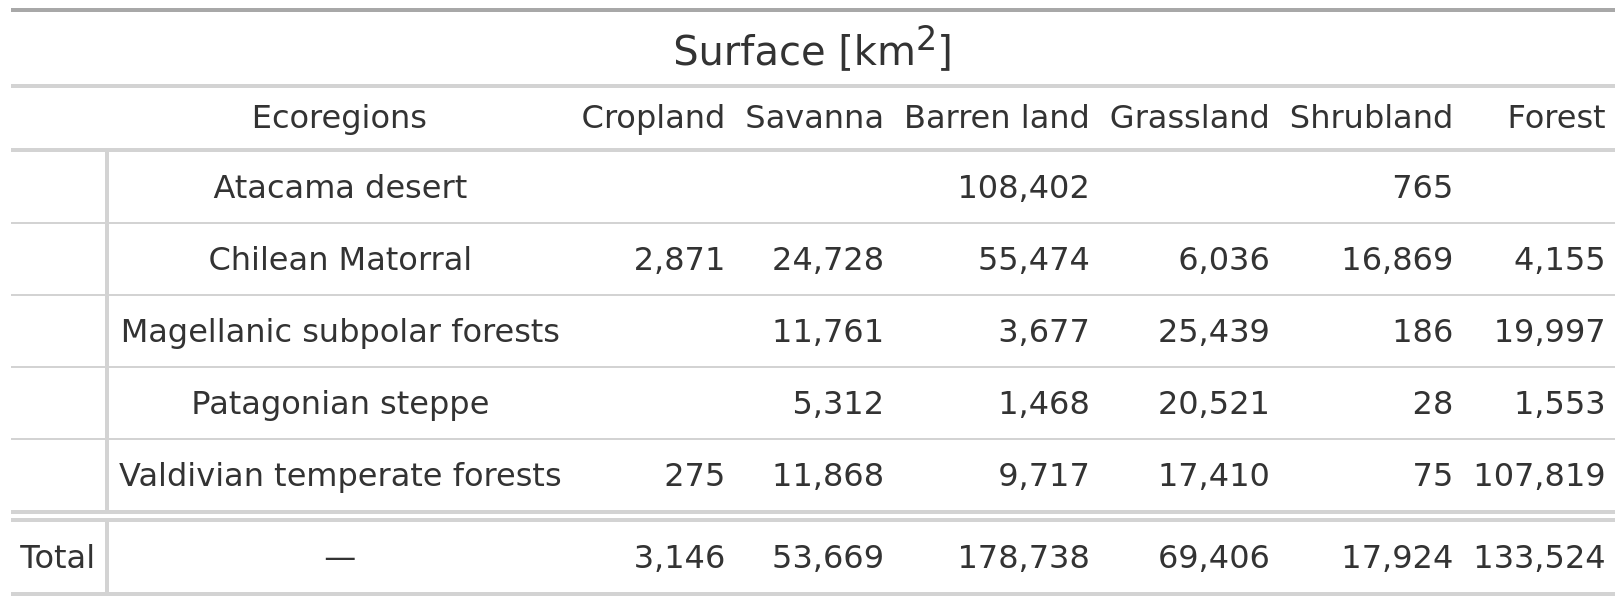
\includegraphics[width = .5\textwidth]{../output/figs/table_surface_landcover_macrozone.png}
\end{table}

\begin{figure}[!ht]

{\centering 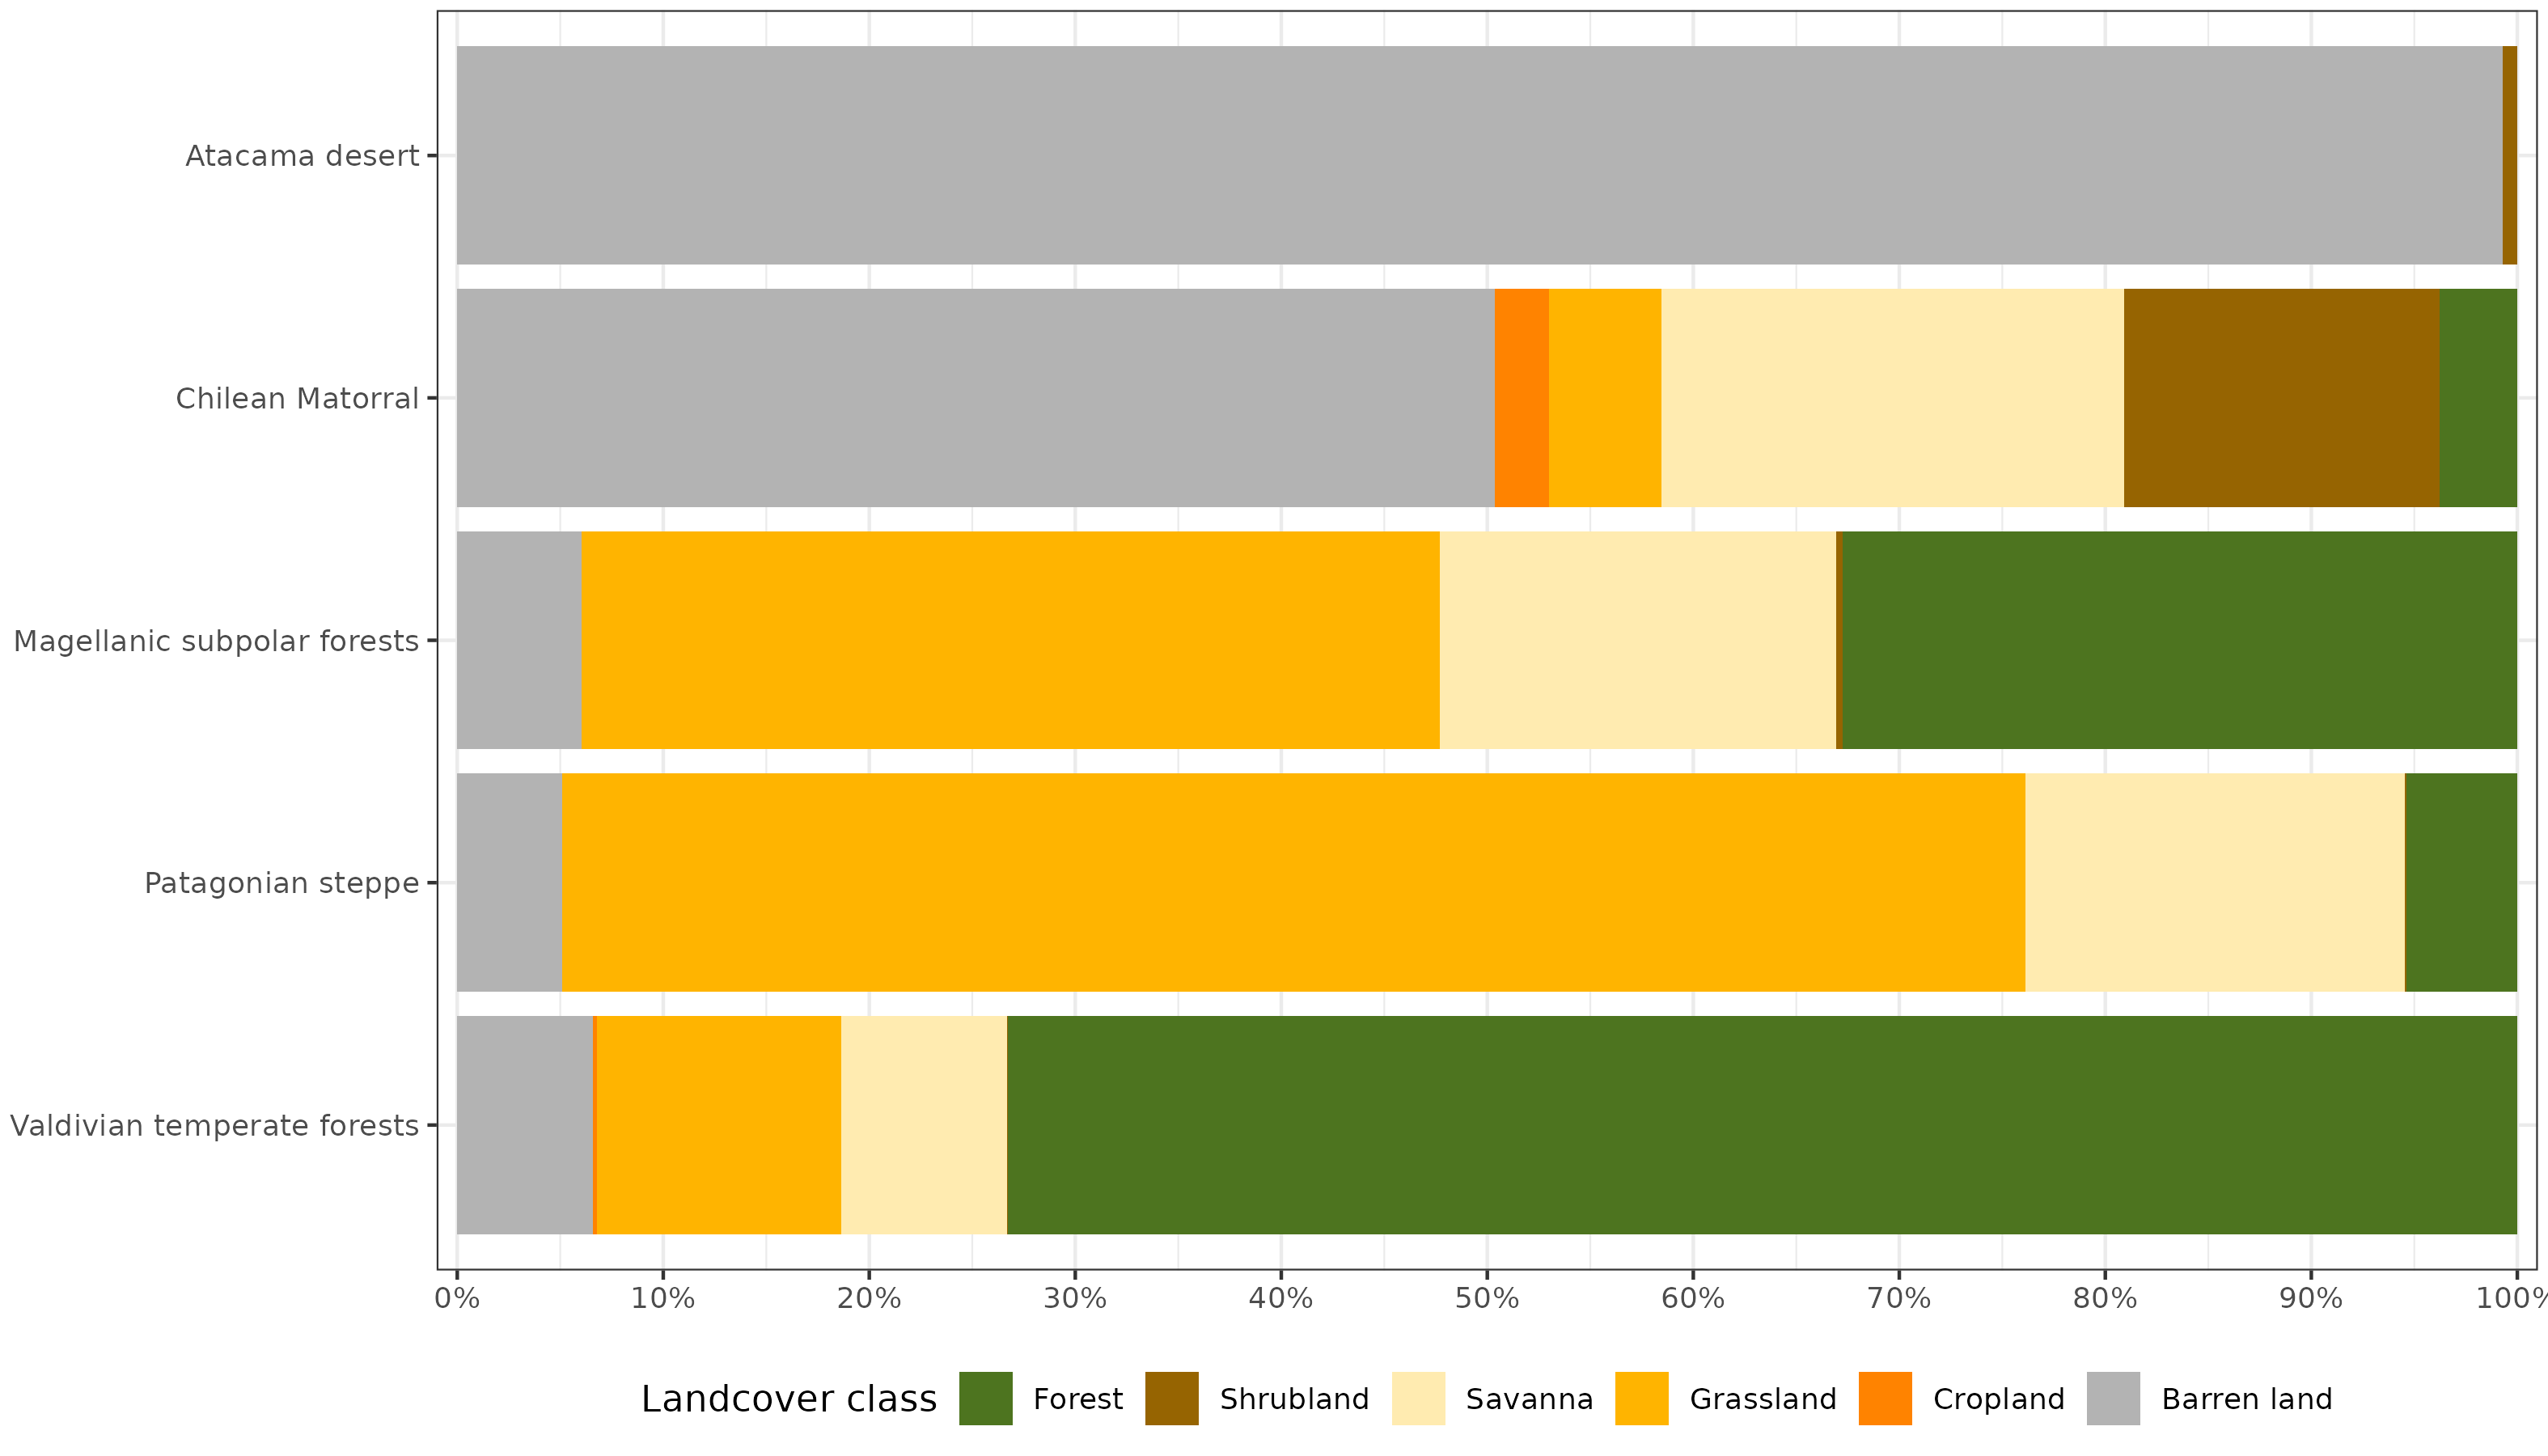
\includegraphics{../output/figs/LC_pers80_per_macrozone.png}

}

\caption{\label{fig-LCprop}Proportion of land cover class from the
persistent land cover for 2001-2022 (\textgreater80\%) per macrozone}

\end{figure}

\hypertarget{land-cover-trend-and-drought-indices-1}{%
\subsubsection{land cover trend and drought
indices}\label{land-cover-trend-and-drought-indices-1}}

\begin{table}[!ht]
\caption{The value of Sen's slope trend next to the time-series plot of surface per land cover class (IGBP MCD12Q1.016) for 2001–2022 through Central Chile. Values of zero indicate that there was not a significant trend. Red dots on the plots indicate the maximum and minimum values of surface.}
\label{tab-land coverTrend}
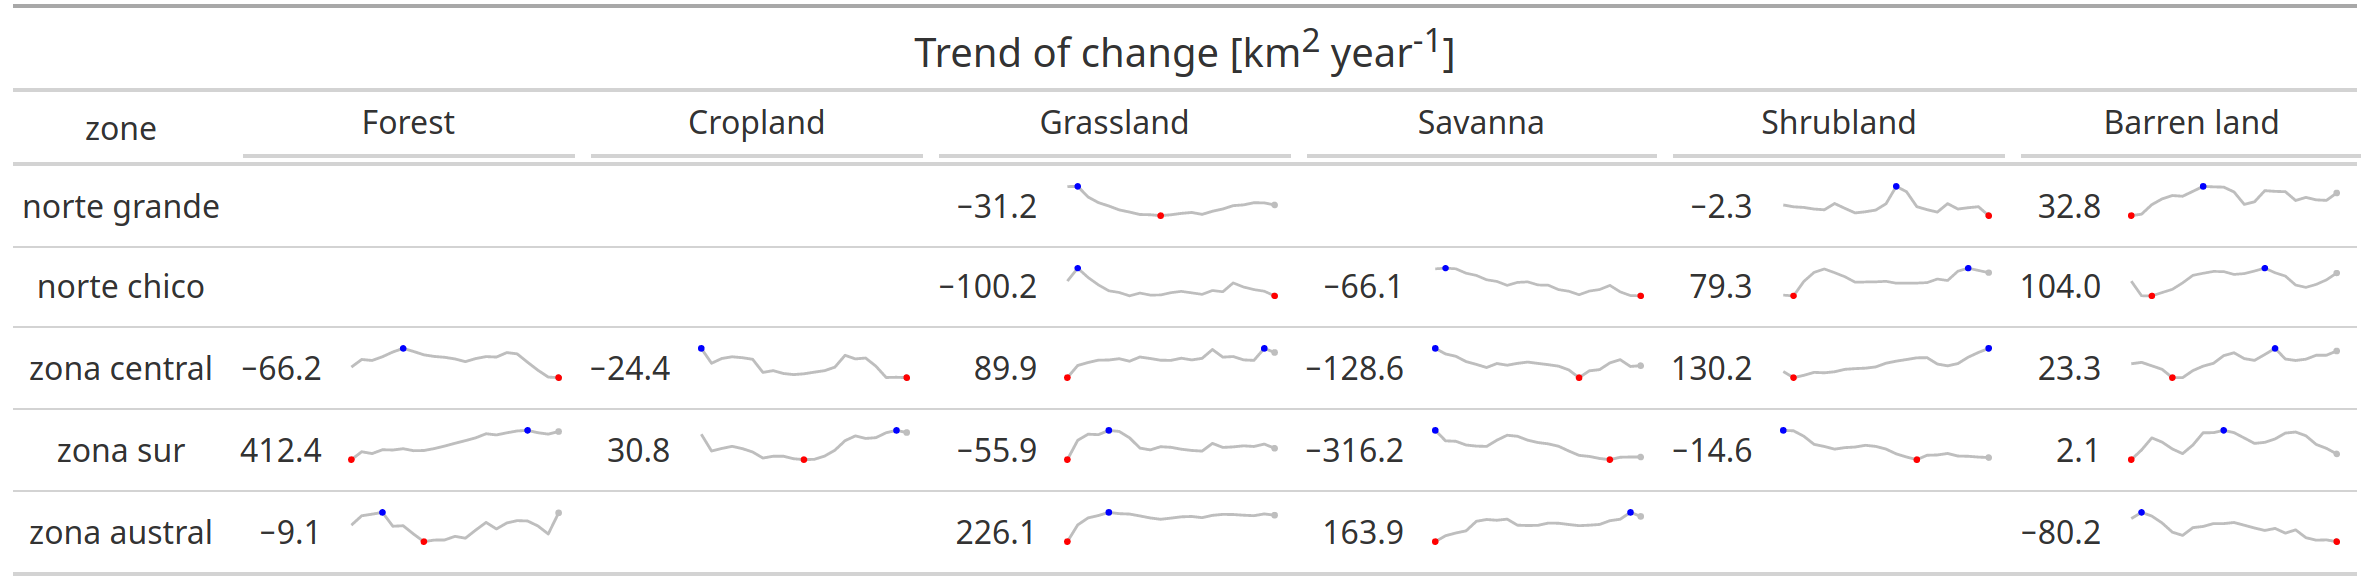
\includegraphics[]{../output/figs/table_var_landcover_macro.png}
\end{table}

The ``Norte Chico'' shows an increase in barrend land of 111
\(km^2 year^{-1}\) and a reduction in the class savanna of 70
\(km^2 year^{-1}\). In the ``Centro'' and ``Sur,'' there are changes in
the Chilean matorral, with an important reduction in savanna (136 to 318
\(km^2 yr^{-1}\)), and an increase in shrubland and grassland. Showing a
change for more dense vegetation types. It appears to be a shift in the
area of cropland from the ``Centro'' to the ``Sur.'' Also, there is a
high increase in forest (397 \(km^2 yr^{-1}\)) in the ``Sur,'' replacing
the savanna lost.

Further, we want to address whether the trend in land cover change for
2001--2023 is associated with trends in drought indices of water demand
and supply and/or soil moisture for macrozone and land cover
macroclasses. From the three methods tested, Ridge, Lasso, and Random
Forest, neither gives significant results regarding whether the trend in
a drought index for any time scale explains the trend in land cover
change. Nevertheless, in ``Norte Chico'' and ``Centro,'' there is a
decrease in croplands and savanna and an increase in barren land, which
is associated with the variation in drought indices. Mainly for a
decrease in water supply (SPI and SSI) and an increase in water demand
(EDDI). However, due to the high variability from north to south in
Chile, the climatic condition (arid, semi-arid, and humid), and the land
cover type, we believe that only in those zones could the LULCC be
driven to some degree by drought.

\hypertarget{trend-of-drought-indices-for-water-demand-and-supply-soil-moisture-and-vegetation-productivity-1}{%
\subsection{Trend of drought indices for water demand and supply, soil
moisture, and vegetation
productivity}\label{trend-of-drought-indices-for-water-demand-and-supply-soil-moisture-and-vegetation-productivity-1}}

\begin{figure}[!ht]

{\centering 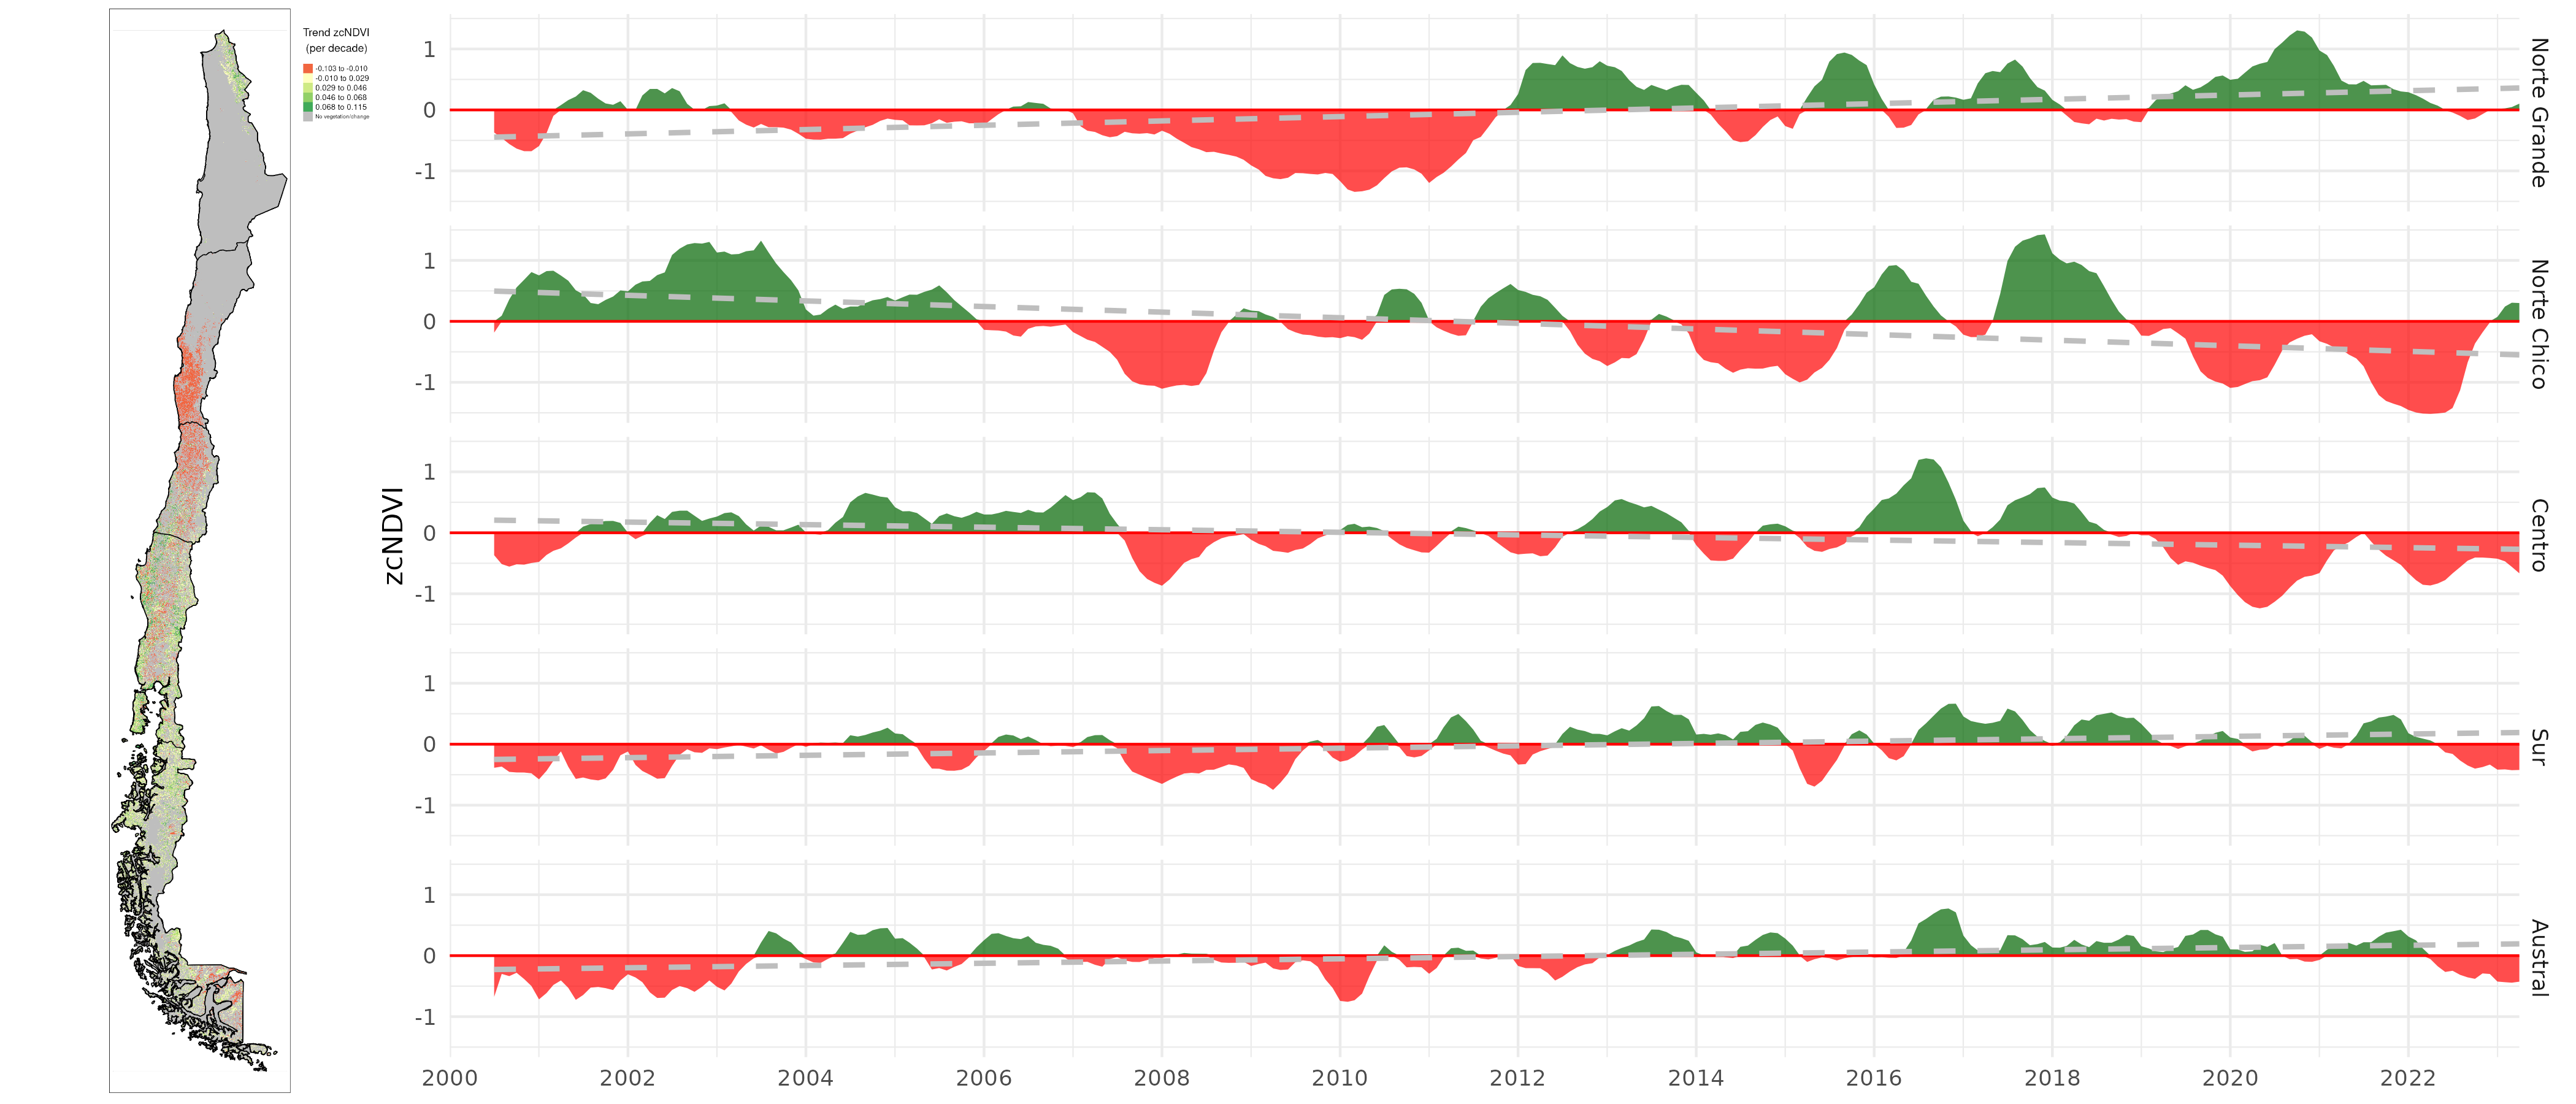
\includegraphics{../output/figs/temporal_variation_zcNDVI6_macrozonas_con_mapa.png}

}

\caption{\label{fig-zcNDVI_var}(a) Map of the linear trend of the index
zcNDVI-6 for 2001--2023. Greener colors indicate a positive trend; reder
colors correspond to a negative trend and a decrease in vegetation
productivity. Grey colors indicate either no vegetation or a change in
land cover type for 2001--2022. (b) Temporal variation of zcNDVI-6
aggregated at macrozone level within continental Chile. Each horizontal
panel corresponds to a macrozone from `Norte Grande' to `Austral'.}

\end{figure}

Regarding vegetation productivity aggregated through the macrozones in
the five land cover macroclasses, in ``Norte Grande,'' there is an
increase trend of 0.02 (z-index) per decade, related to types of
grassland and shrubland. There is a negative trend in ``Norte Chico''
with -0.04 and ``Centro'' with -0.02 per decade. In the ``Norte Chico,''
savanna (-0.05) has the lowest trend, and the rest of the types are
around -0.04. In ``Centro,'' shrubland reaches -0.06, grassland -0.05,
and croplands and savanna -0.01 per decade. This could be associated
either with a reduction in vegetation surface, a decrease in biomass, or
browning \citep{Miranda2023}. Vegetation reached its lowest values since
the year 2019, reaching an extreme condition in early 2020 and 2022 in
the ``Norte Chico'' and Centro'' (Mega Drought). The ``Sur'' and
``Austral'' show a positive trend of around 0.016 per decade
(Figure~\ref{fig-zcNDVI_var}). Despite the croplands suffering from
drought just as badly as the native vegetation in ``Norte Chico,'' the
Chilean matorral appears to be the region most affected by a negative
trend in vegetation \citep{Fuentes2021}.

\begin{figure}[!ht]

{\centering 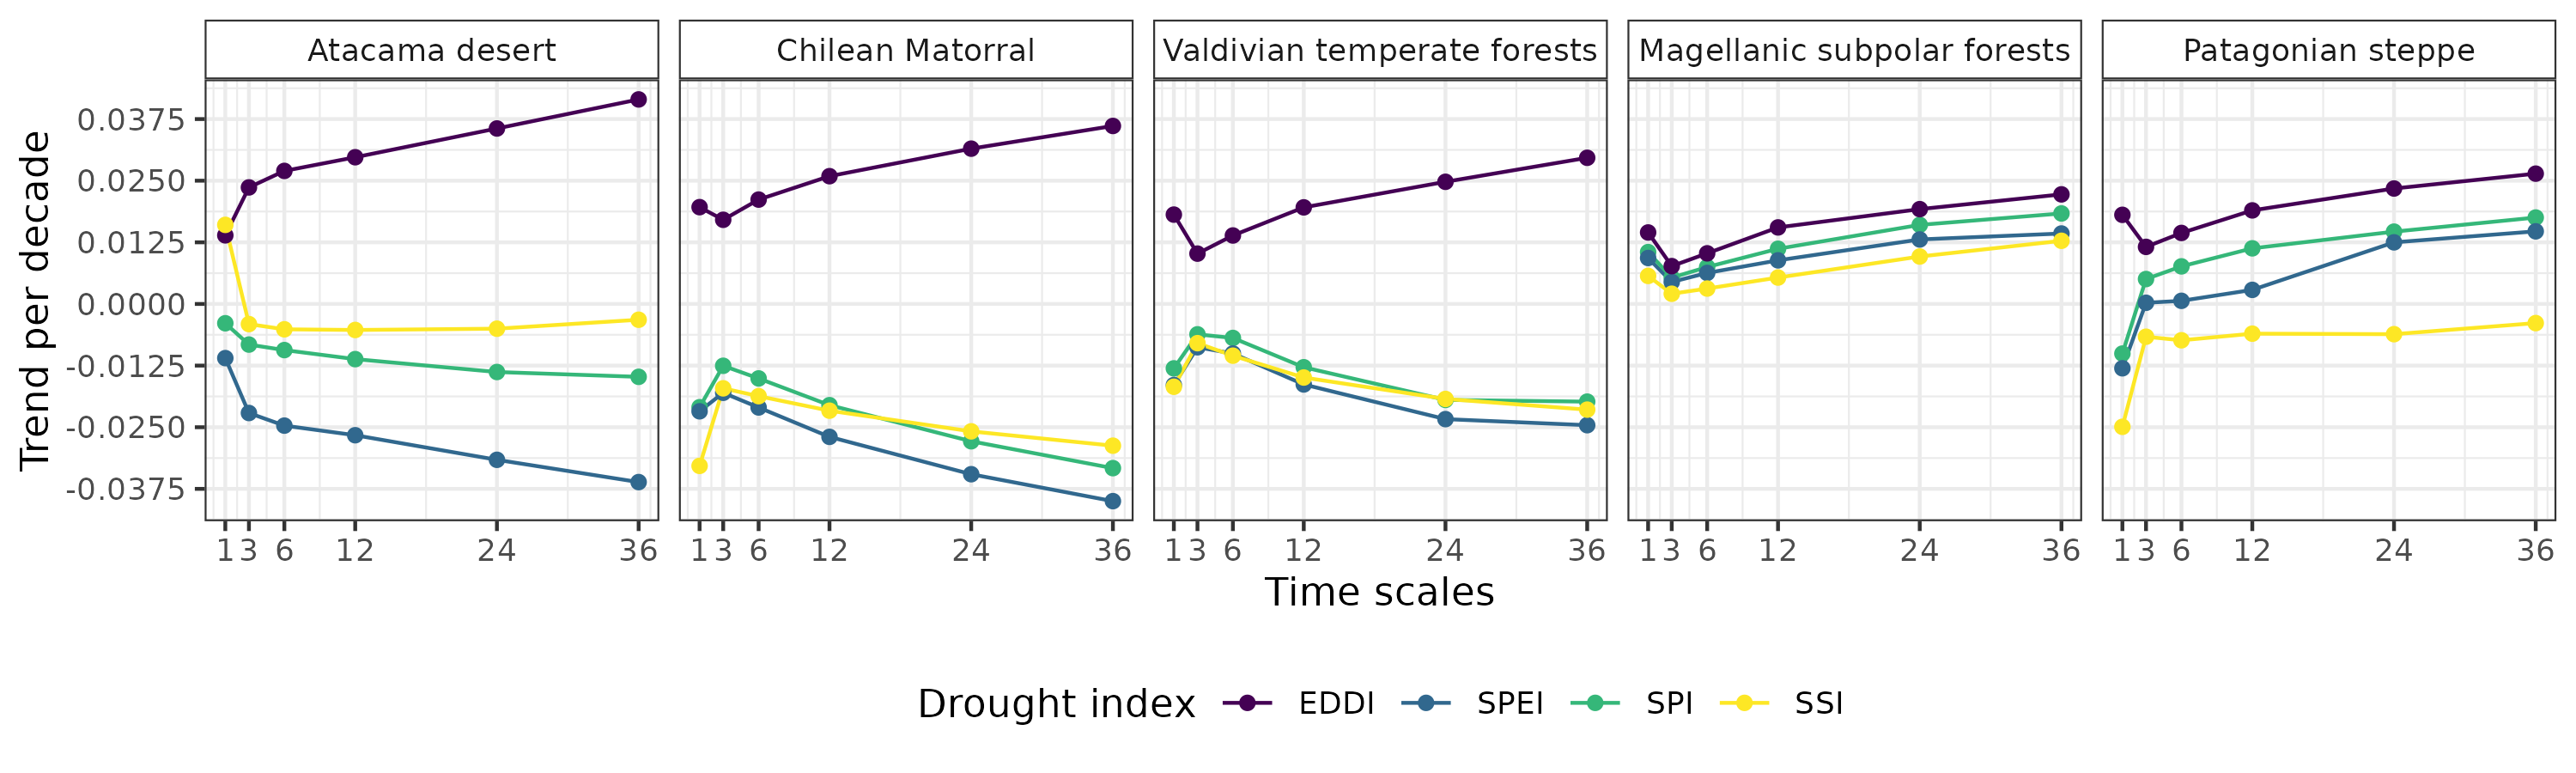
\includegraphics{../output/figs/trend_macrozone_drought_indices.png}

}

\caption{\label{fig-trendDIMacro}Trend per decade for the drought
indices SPI, EDDI, SPEI, and SSI aggregated by macrozone.}

\end{figure}

Analyzing the water supply, the macrozones that have the lowest trend
are ``Norte Chico'' and ``Centro,'' where the SPI, SPEI, and SSI show
that it decreases at longer time scales due to the prolonged reduction
in precipitation. At 36 months, it reaches trends between -0.03 and
-0.04 (z-score) per decade for SPI, SPEI, and SSI
(Figure~\ref{fig-trendDI}). For ``Sur,'' the behavior is similar,
decreasing at longer scales and having between -0.016 and -0.025 per
decade for SPI, SPEI, and SSI. On the other hand, all macrozones show an
increase in the trend in all the drought indices, with ``Norte Grande''
having the highest at 36 months (0.042 per decade). Because of this, the
SPEI (which uses AED) reached its lowest value in ``Norte Grande,'' with
-0.03 at 36 months. Despite the other macrozones, ``Austral'' showed an
increase in all indices, being the highest for EDDI at 36 months (0.025)
and the lowest for SSI, which shows only a minor increase in the trend
(Figure~\ref{fig-trendDI} and Figure~\ref{fig-trendDIMacro}).

\hypertarget{impact-for-water-supply-and-demand-and-soil-moisture-in-vegetation-productivity}{%
\subsection{Impact for water supply and demand, and soil moisture in
vegetation
productivity}\label{impact-for-water-supply-and-demand-and-soil-moisture-in-vegetation-productivity}}

According to what is shown in Figure~\ref{fig-corTimeScale},
Figure~\ref{fig-corPerson}, and Table \ref{tab-corland cover}, forest
seems to be the most resistant type to drought. Showing that only
``Centro'' is slightly (rsq = 0.25) impacted by a 12-month soil moisture
deficit (SSI-12). In the ``Norte Chico'' and to a lesser extent in the
``Norte Grande,'' it is evident that a SSI-12 with a rsq = 0.45 and a
decrease in water supply (SPI-36 and SPEI-24 with rsq = 0.28 and 0.34,
respectively) have an impact on grasslands. However, this type was
unaffected by soil moisture, water supply, or demand in macrozones
further south. The types that show to be most affected by variation in
climate conditions are shrublands, savannas, and croplands. For savannas
in ``Norte Chico,'' the SSI-12 and SPI-24 reached an rsq of 0.74 and
0.58, respectively. This value decreases to the south, but the SSI-12 is
still the variable explaining more of the variation in vegetation
productivity (rsq = 0.45 in ``Centro'' and 0.2 in ``Sur''). In the case
of croplands, the SPEI-12, SPI-36, and SSI-12 explain between 45\% and
66\% of ``Norte Chico.'' The type of land most impacted by climatic
variation was shrubland, where soil moisture explained 59\% and
precipitation, 37\%, in ``Norte Chico'' and ``Centro,'' with SSI-12
being the most relevant variable, then SPI-36 in ``Norte Chico'' and
SPI-24 in ``Sur.''

\newpage

\blandscape

\begin{figure}

\begin{minipage}[t]{0.50\linewidth}

{\centering 

\raisebox{-\height}{

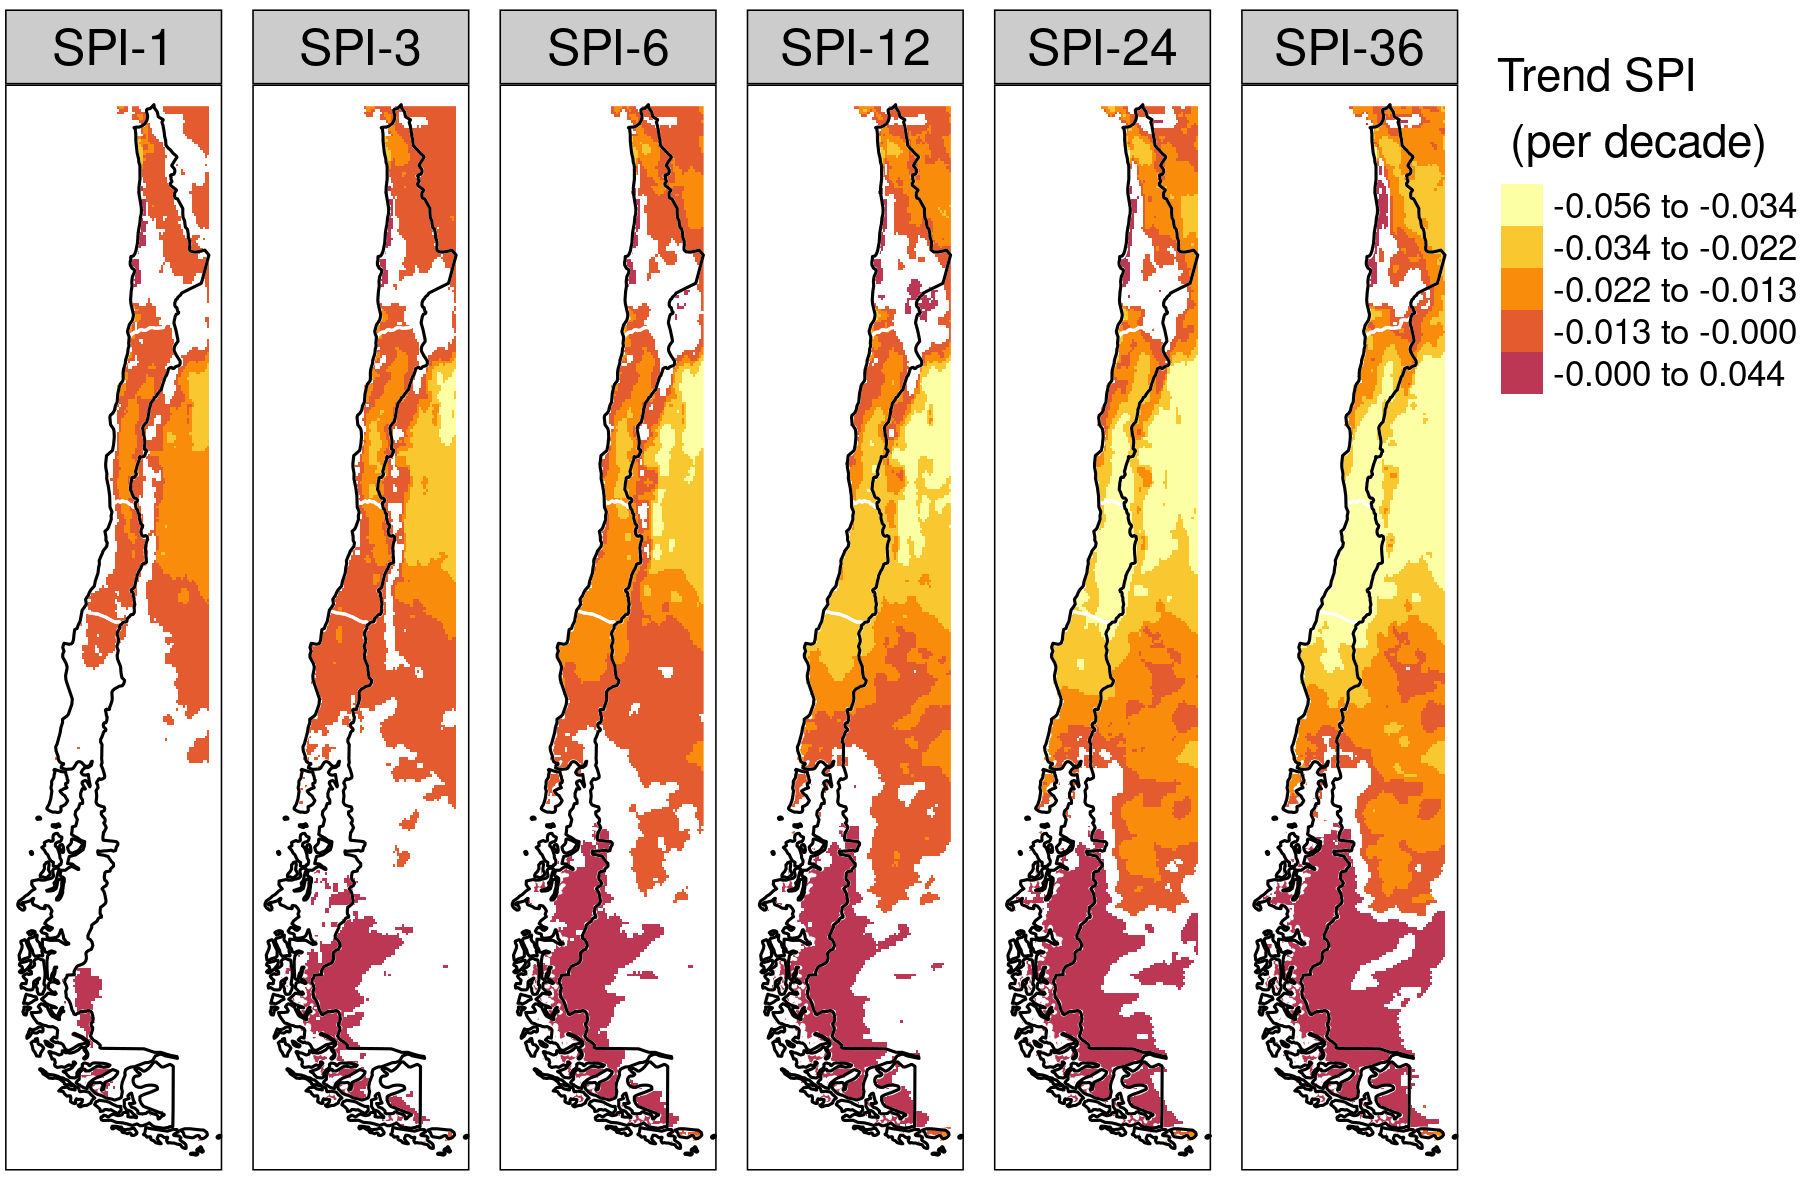
\includegraphics{../output/figs/trend_raster_SPI_1981-2023.png}

}

}

\subcaption{\label{fig-trendDI-1}SPI (Standardized Precipitation Index)}
\end{minipage}%
%
\begin{minipage}[t]{0.50\linewidth}

{\centering 

\raisebox{-\height}{

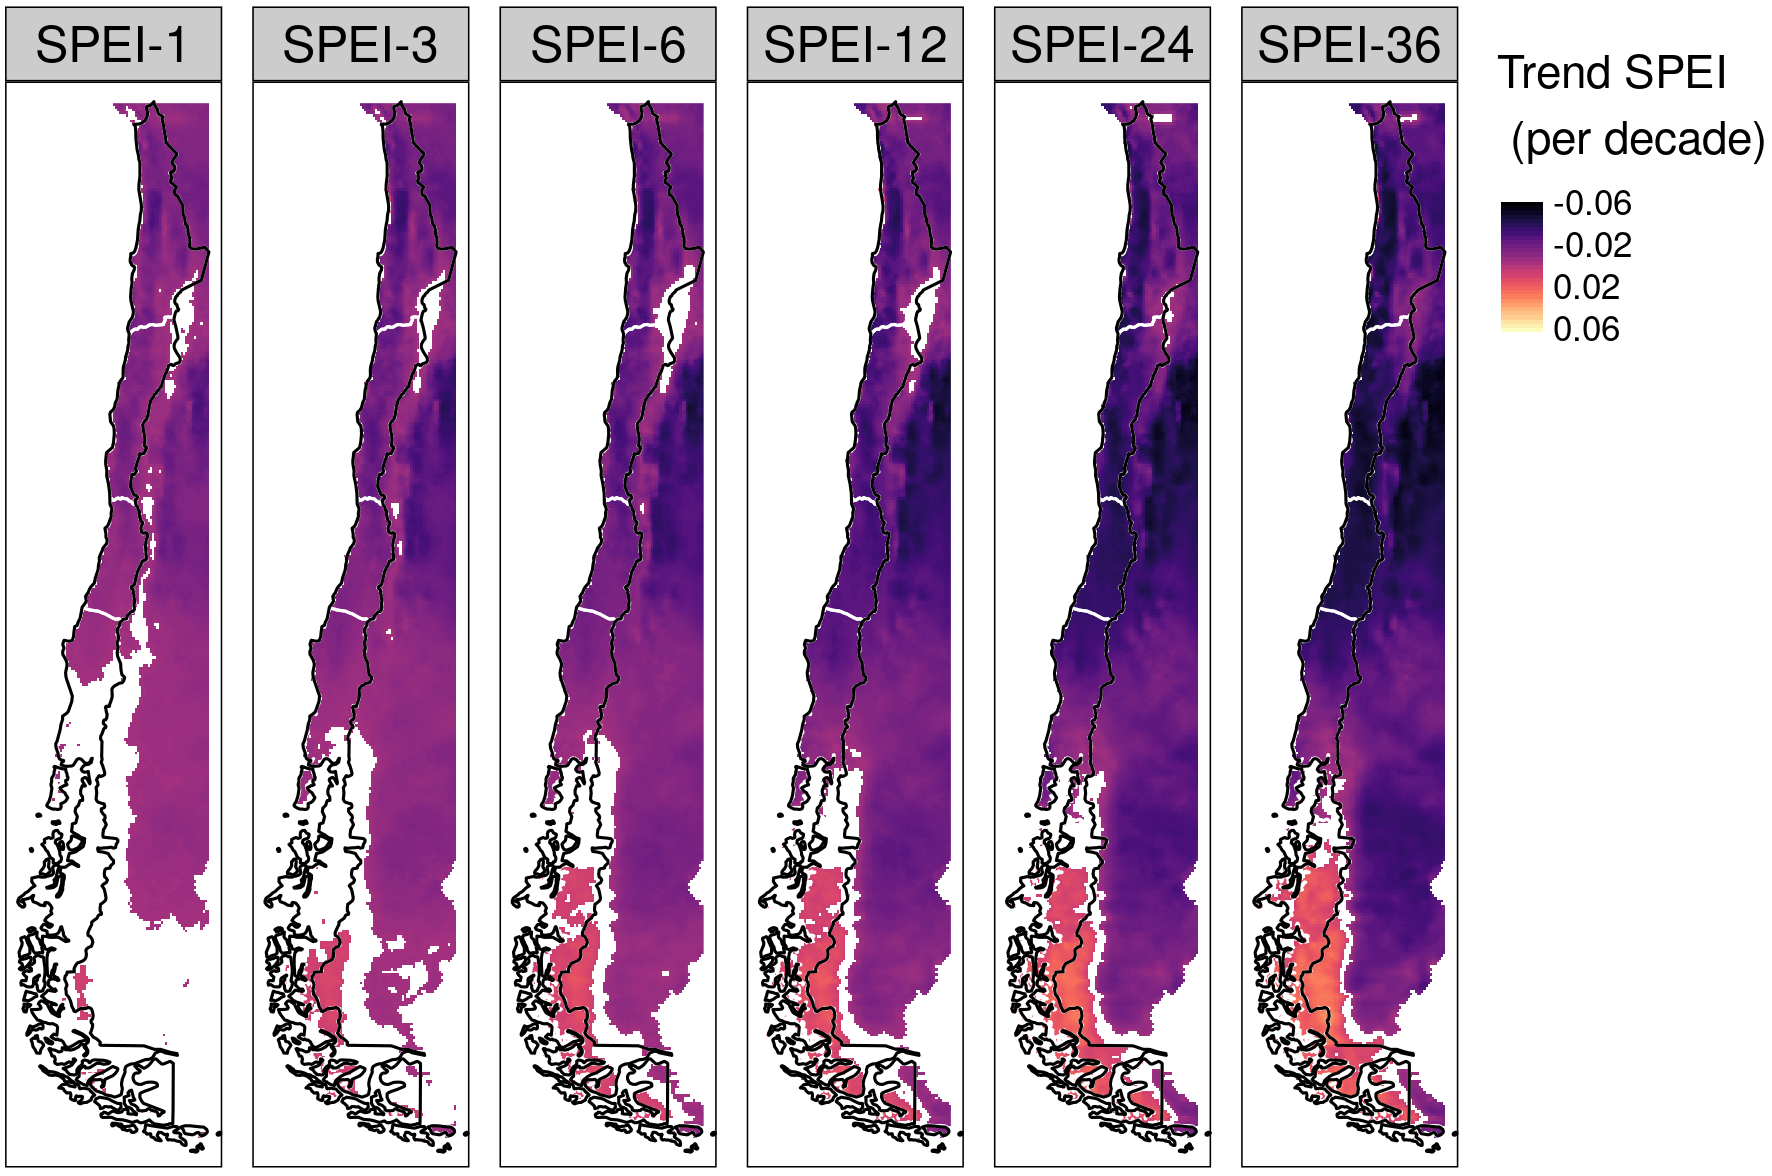
\includegraphics{../output/figs/trend_raster_SPEI_1981-2023.png}

}

}

\subcaption{\label{fig-trendDI-2}SPEI (Standardized Precipitation
Evapotranspiration Index)}
\end{minipage}%
\newline
\begin{minipage}[t]{0.50\linewidth}

{\centering 

\raisebox{-\height}{

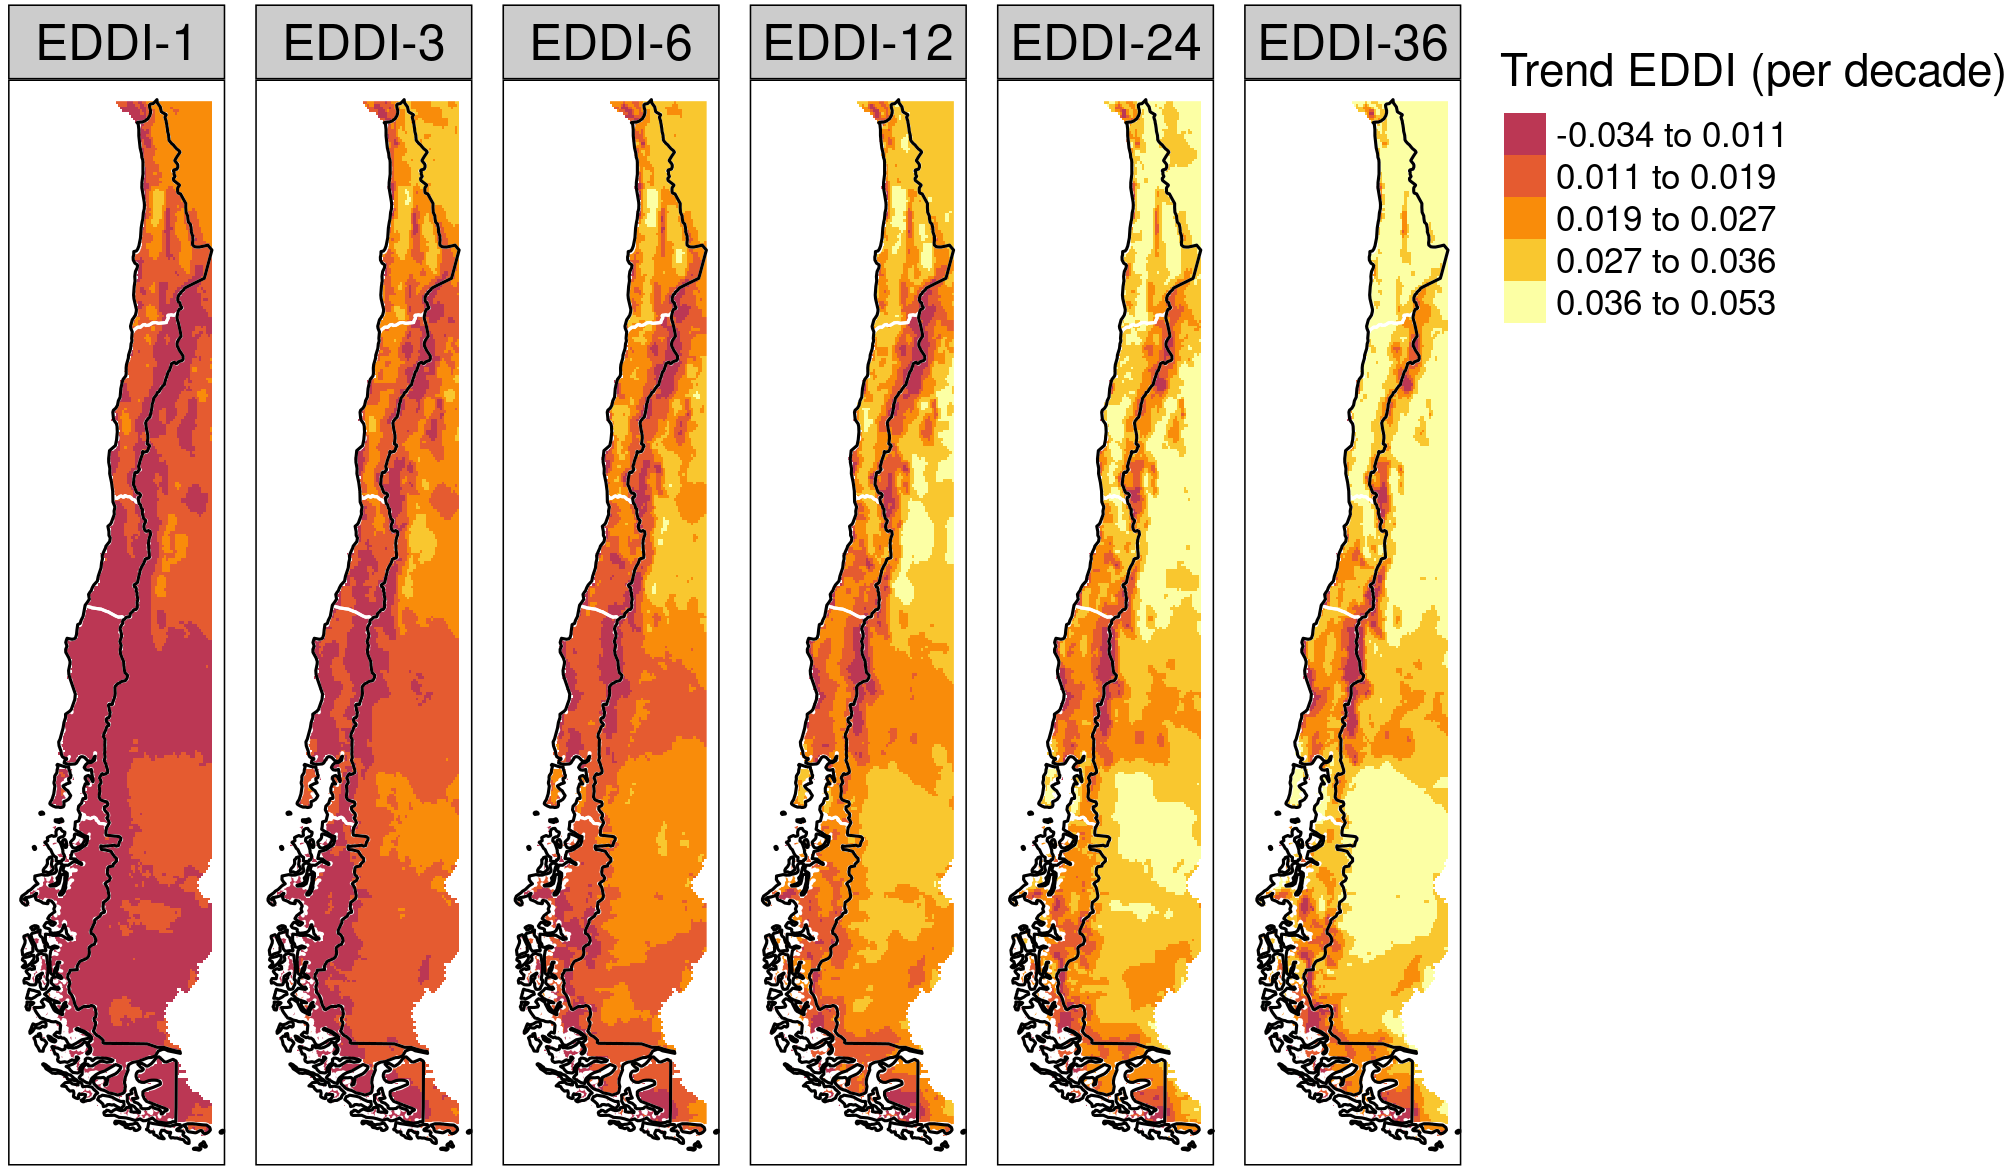
\includegraphics{../output/figs/trend_raster_EDDI_1981-2023.png}

}

}

\subcaption{\label{fig-trendDI-3}EDDI (Evaporative Demand Drought
Index)}
\end{minipage}%
%
\begin{minipage}[t]{0.50\linewidth}

{\centering 

\raisebox{-\height}{

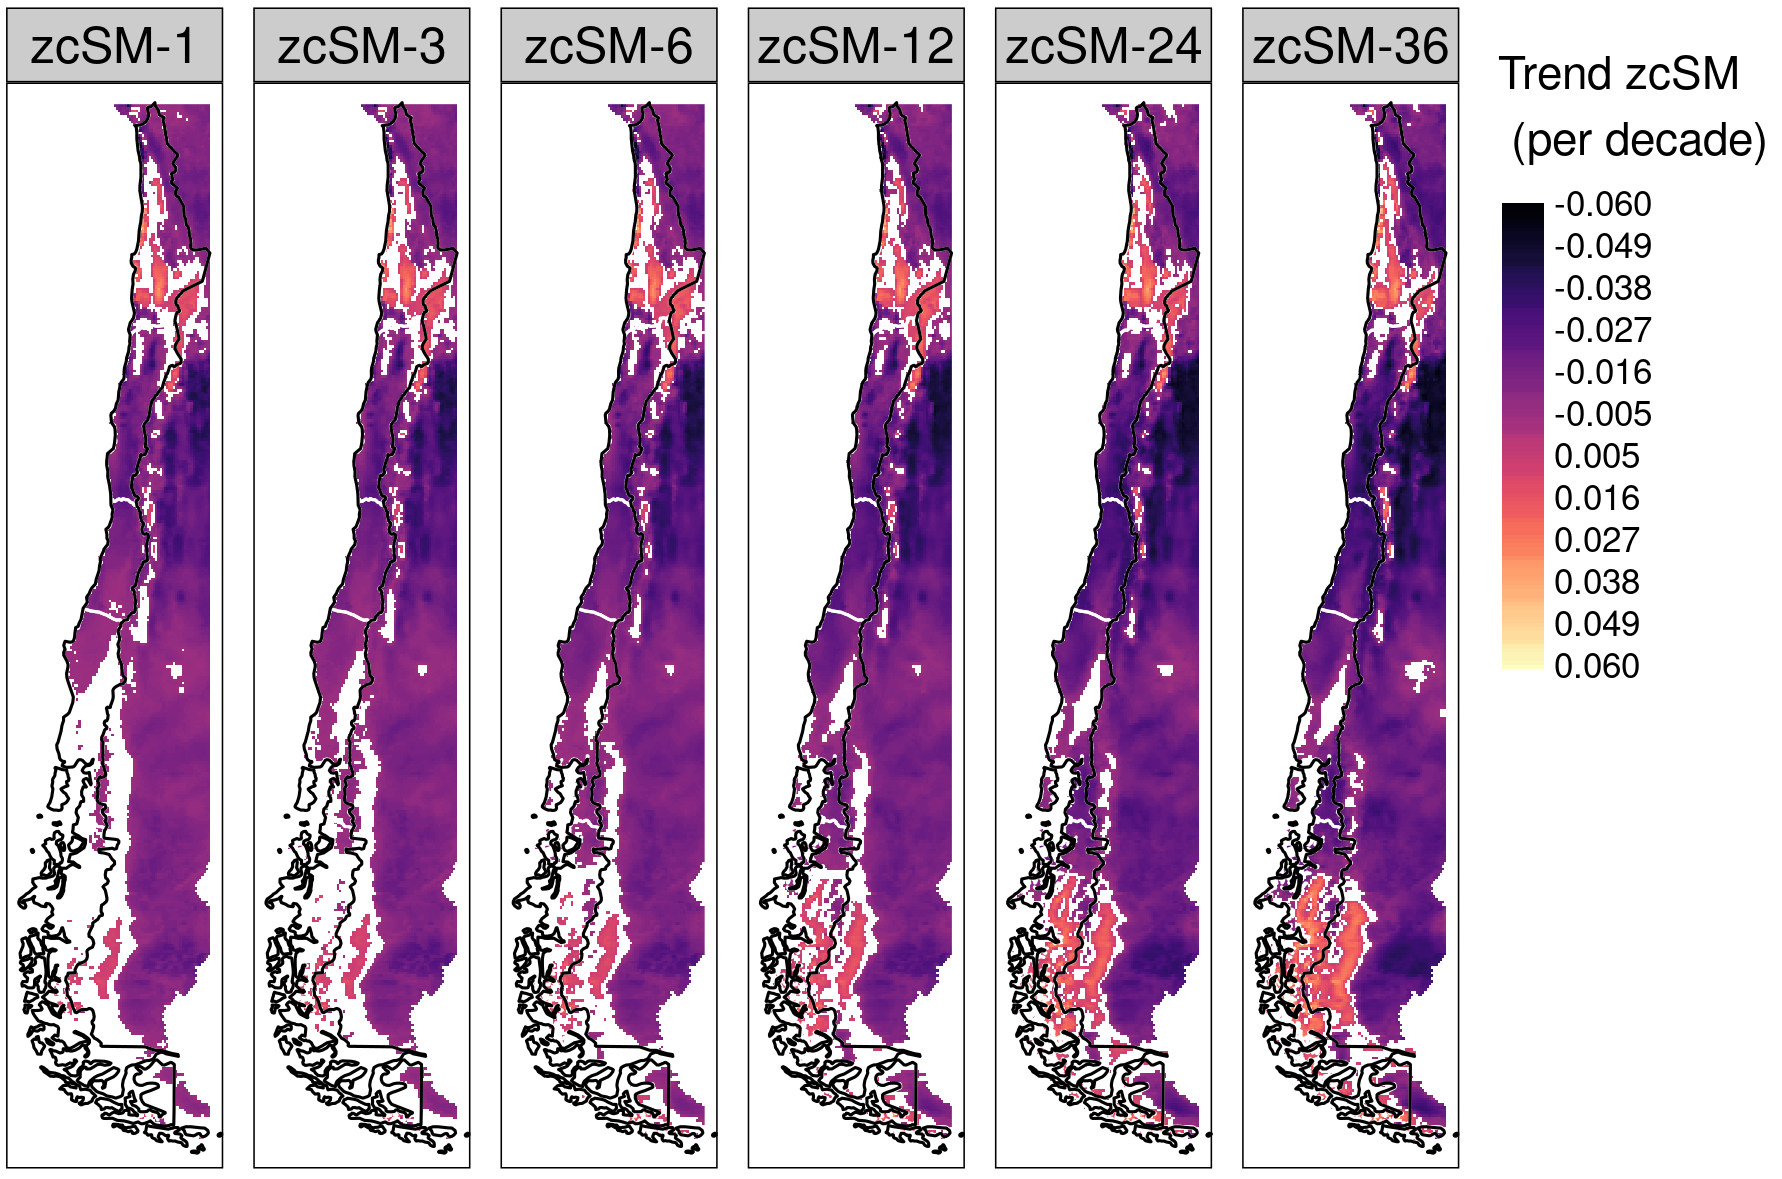
\includegraphics{../output/figs/trend_raster_zcSM_1981-2023.png}

}

}

\subcaption{\label{fig-trendDI-4}SSMI (Standardized Soil Moisture
Index)}
\end{minipage}%

\caption{\label{fig-trendDI}Linear trend of the drought index (*) at
time scales of 1, 3, 6, 12, 24, and 36 months for 1981-2023}

\end{figure}

\elandscape

\begin{table}[!ht]
\caption{Summarry per land cover macroclass and macrozone regarding the correlation between zcNDVI with the drought indices EDDI, SPI, SPEI, and SSI for time scales of 1, 3, 6, 12, 24, and 36. The numbers in each cell indicate the time scale that reached the maximum correlation for the land cover and macrozone, and the color indicates the strength of the r-squared obtained with the index and the time scale.}
\label{tab-corland cover}
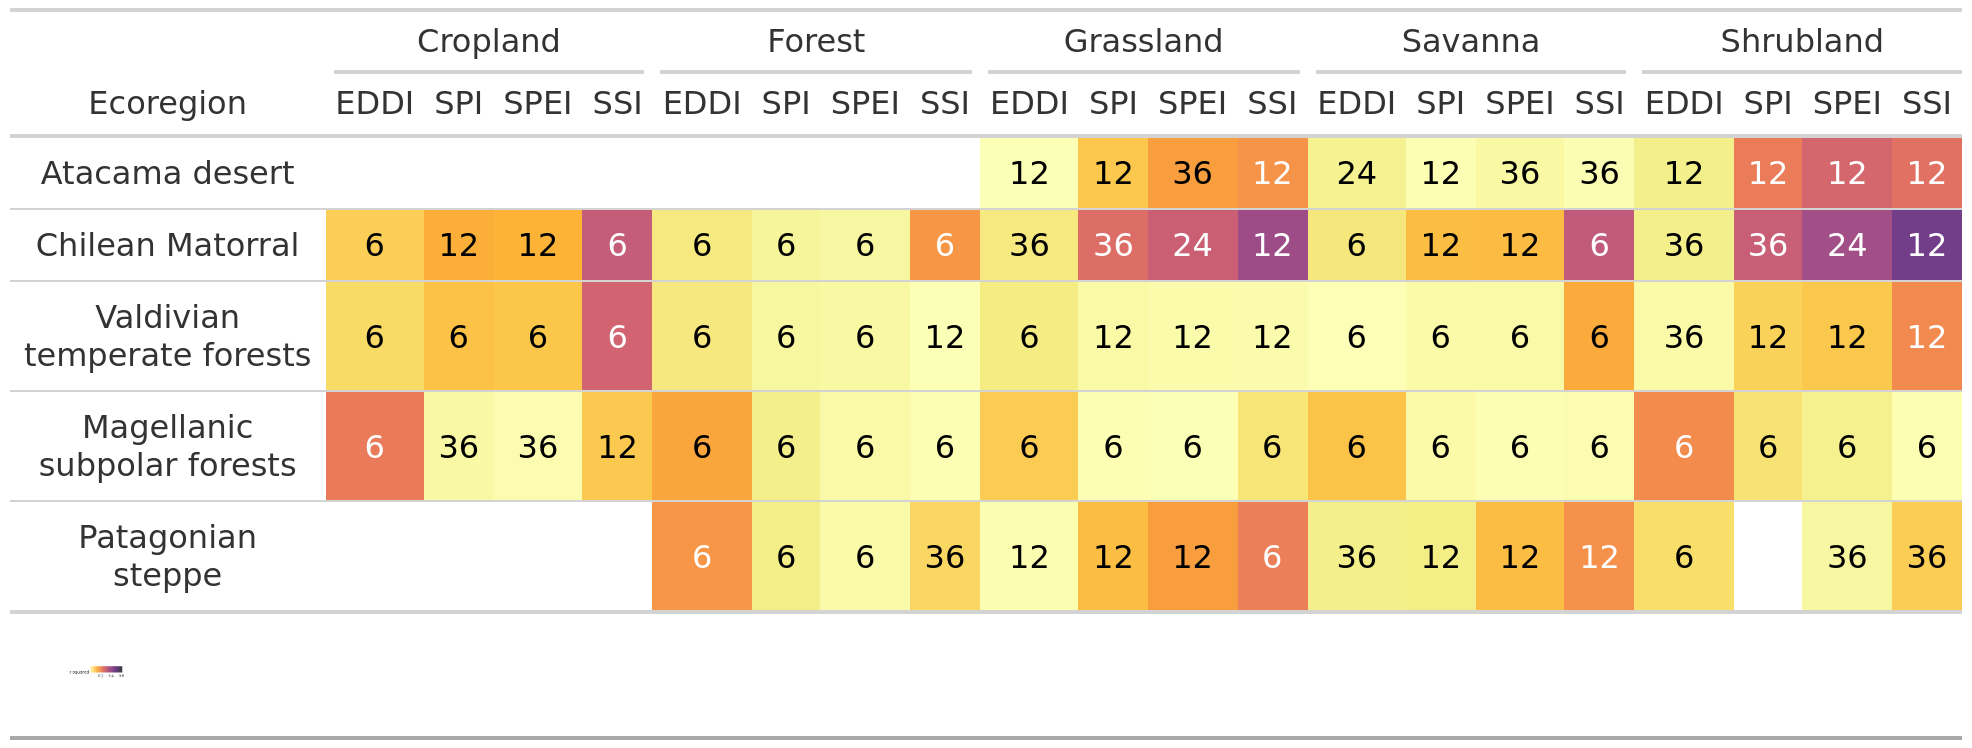
\includegraphics[]{../output/figs/tabla_r_cor_macro_indice.png}
\end{table}

\begin{figure}[!ht]

{\centering 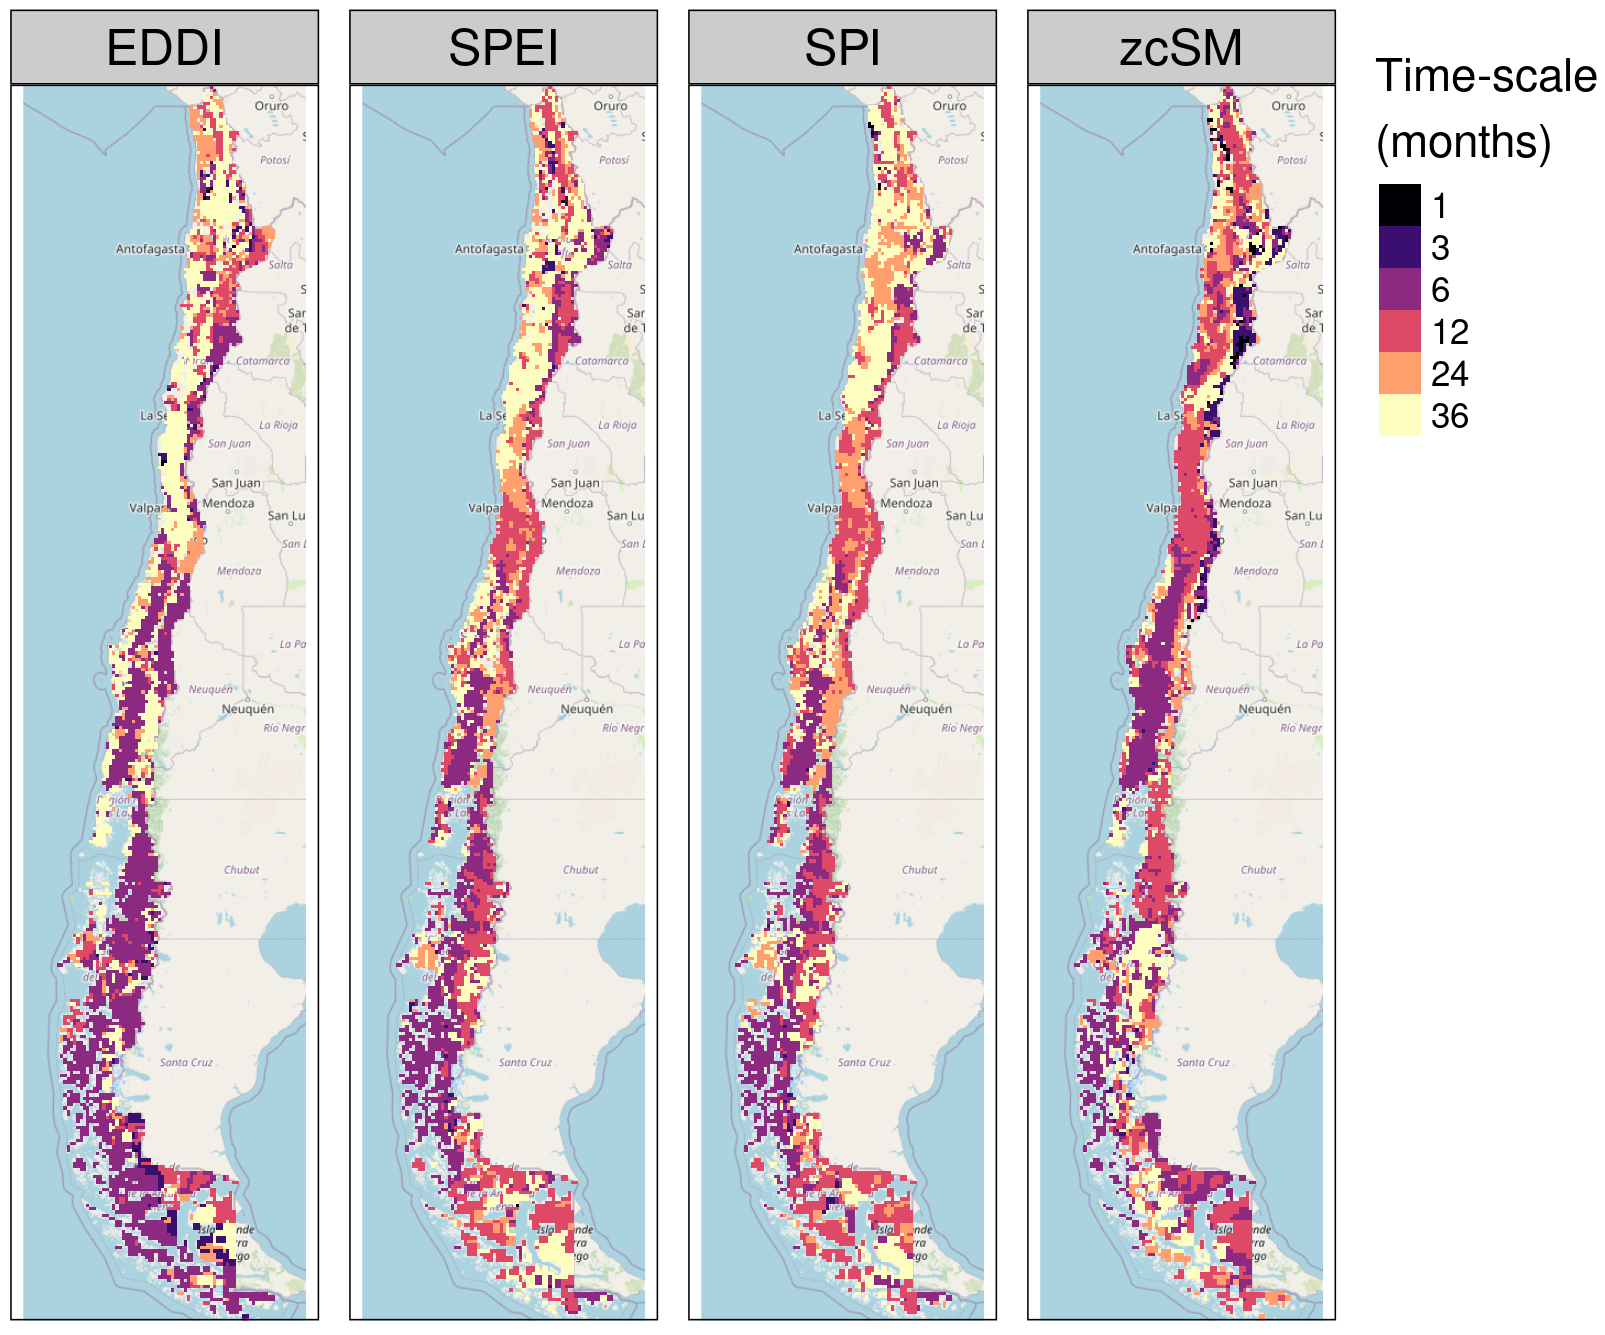
\includegraphics{../output/figs/mapa_cor_selec_indices_zcNDVI6.png}

}

\caption{\label{fig-corTimeScale}Time scales per drought index that
reach the maximum coefficient of determination}

\end{figure}

\begin{figure}[!ht]

{\centering 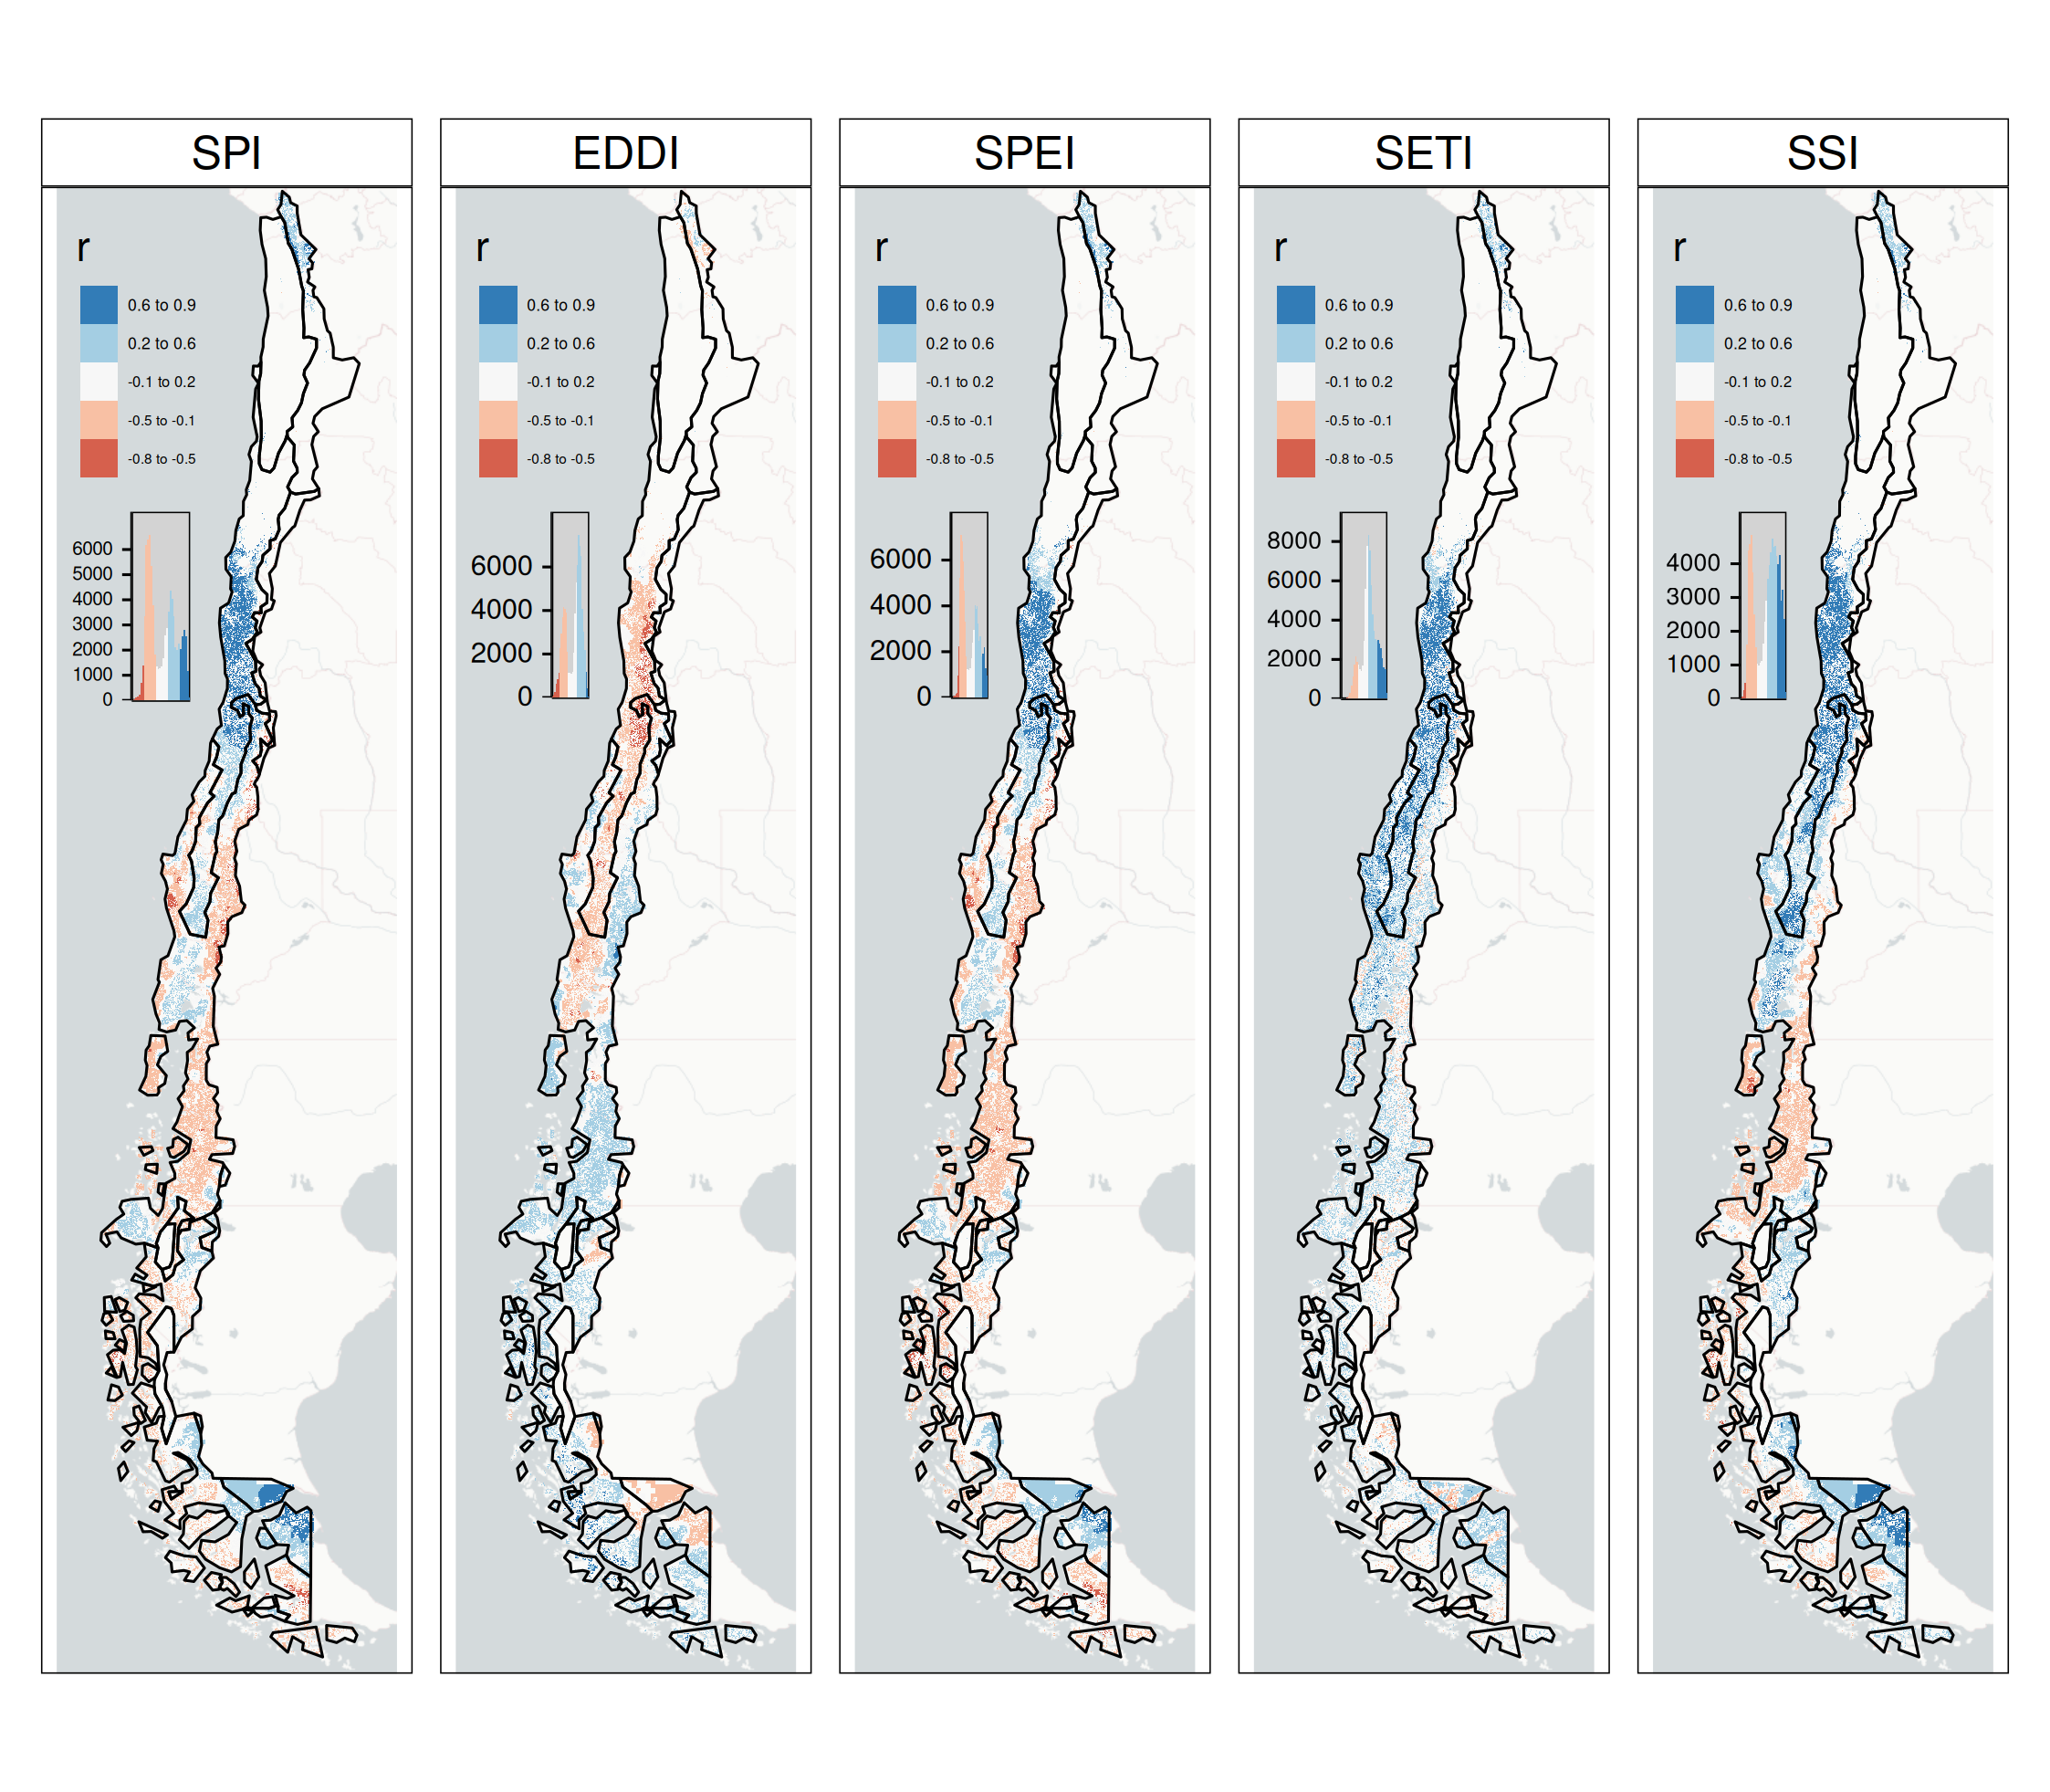
\includegraphics{../output/figs/mapa_cor_r_indices_zcNDVI6.png}

}

\caption{\label{fig-corPerson}Pearson correlation value for the time
scales and drought index that reach the maximum coefficient of
determination}

\end{figure}

\hypertarget{discussion}{%
\section{Discussion}\label{discussion}}

\hypertarget{ecological-and-agricultural-drought}{%
\subsection{Ecological and agricultural
drought}\label{ecological-and-agricultural-drought}}

\hypertarget{drought-trend-lulcc-and-climate-conditions}{%
\subsection{Drought trend, LULCC, and climate
conditions}\label{drought-trend-lulcc-and-climate-conditions}}

1.- Respecto a lo que indica \citet{Vicente-Serrano2018}, de que el
aumento en la tendencia en severidad de la sequía (hidrológica) tiene
que ver más con un aumento de la demanda de agua (ej, LULCC, amazonas)
que a una tendencia en las condiciones climáticas (SPI-12). ¿Qué pasa en
Chile?

\hypertarget{land-cover-types-most-impacted-by-drought-throughout-chile}{%
\subsection{land cover types most impacted by drought throughout
Chile}\label{land-cover-types-most-impacted-by-drought-throughout-chile}}

2.- Sobre los tipos de land cover más afectados por los indicadores de
sequía. Asociación con el matorral chileno \citep{Fuentes2021}.
Diferencia entre el Norte Chico, Centro y lo que pasa hacía el sur.

\hypertarget{drought-indices-of-water-demand-and-supply-soil-moisture-to-predict-changes-in-vegetation-productivity}{%
\subsection{Drought indices of water demand and supply, soil moisture to
predict changes in vegetation
productivity}\label{drought-indices-of-water-demand-and-supply-soil-moisture-to-predict-changes-in-vegetation-productivity}}

\begin{enumerate}
\def\labelenumi{\arabic{enumi}.}
\setcounter{enumi}{2}
\tightlist
\item
  Como podrían servir estos resultados para desarrollar o mejorar un
  predictor de productividad de la vegetación.
\end{enumerate}

\begin{itemize}
\tightlist
\item
  Los datos ERA5L están casi en tiempo real, 7 dias; MODIS también.
\item
  EL SSI se ve como un poderoso indicador que explica la variabilidad en
  la productividad de la vegetación.
\end{itemize}

\hypertarget{future-outlook}{%
\subsection{Future outlook}\label{future-outlook}}

4.- Qué se podría hacer mejor en futuras investigaciones del tema. -
mejorar la resolución y calidad de los datos climáticos -

\hypertarget{conclusion}{%
\section{Conclusion}\label{conclusion}}

\newpage


\renewcommand\refname{References}
  \bibliography{references.bib}


\end{document}
